\documentclass[fleqn]{summary}

\title{Graph Theory Summary}
\author{Jens Ochsenmeier}

\begin{document}

  % \section{Intro to C}

\textbf{Hello World}
\lstinputlisting[style=customc]{hello.c}
\begin{items}
  \item \code{#include}: preprocessor inserts \code{stdio.h} contents
  \item \code{stdio.h}: contains \code{printf} declaration
  \item \code{main}: program starts here
  \item \code{void}: keyword for argument absence
  \item \code{\{  \}}: basic block/scope delimiters
  \item \code{printf}: prints to the terminal
  \item \code{\\n}: newline character
  \item \code{return}: leave function, return value
\end{items}

\textbf{Compiling}
\begin{lstlisting}[style=custombash]
  $ gcc hello.c -o hello
  $ ./hello
  Hello World!
\end{lstlisting}

\textbf{Basic Data Types}
\begin{items}
  \item \code{char c = 5; char c = 'a';} \\*
    one byte, usually for characters (1970: ASCII is fine)
  \item \code{int i = 5; int i = 0xf; int i = 'a';} \\*
    usually 4 bytes, holds integers
  \item \code{float f = 5; float f = 5.5;} \\*
    4 bytes floating point number
  \item \code{double d = 5.19562} \\*
    8 bytes double precision floating point number
\end{items}

\textbf{Basic Data Types -- logic}
\begin{items}
  \item \code{int i = 5 / 2; // i = 2} \\*
    integer logic, no rounding
  \item \code{float f = 5.0f / 2; // f = 2.5f} \\*
    decimal logic for float and double
  \item \code{char a = 'a' / 2 // a = 97 / 2 = 48} \\*
    \code{char} interpreted as character by console
\end{items}

\textbf{Basic Data Types -- signed/unsigned}
\begin{items}
  \item \code{signed int i = -5 // i = -5} (two's complement)
  \item \code{unsigned int i = -5 // i = 4294967291}
\end{items}

\textbf{Basic Data Types -- short/long}
\begin{items}
  \item \code{short int i = 1024 // -32768...32767}
  \item \code{long int i = 1024 // -2147483648...2147483647}
\end{items}

\textbf{Basic Data Types -- more size stuff}
\begin{items}
  \item \code{sizeof int; sizeof long int; // 4; 4;} (x86 32-Bit)
  \item use data types from \code{inttypes.h} to be sure about sizes:
  \begin{lstlisting}[style=customc]
#include <inttypes.h>
int8_t i; uint32_t j;
  \end{lstlisting}
\end{items}

\textbf{Basic Data Types -- const/volatile}
\begin{items}
  \item \code{const int c = 5;} \\*
    \code{i} is constant, changing it will raise compiler error
  \item \code{volatile int i = 5;} \\*
    \code{i} is volatile, may be modified elsewhere (by different program in shared memory, important for CPU caches, register, assumptions thereof)
\end{items}

\newpage

\textbf{Variables -- local vs. global}
\begin{lstlisting}[style=customc]
int m; // global variable

int myroutine(int j) {
  int i = 5 // local variable
  i = i+j;
  return i;
}
\end{lstlisting}
\begin{items}
  \item \emph{global variables} (\code{int m}): \\*
    lifetime: while program runs \\*
    placed on pre-defined place in memory
  \item basic block/function-local variables (\code{int i}): \\*
    lifetime: during invocation of routine \\*
    placed on stack or in registers
\end{items}

\textbf{Variables -- local vs. static}
\begin{lstlisting}[style=customc]
int myroutine(int j) {
  static int i = 5;
  i = i+j;
  return i;
}

k = myroutine(1); // k = 6
k = myroutine(1); // k = 7
\end{lstlisting}
\begin{items}
  \item static function-local variables: \\*
    saved like global variables \\*
    variable persistent across invocations \\*
    lifetime: like global variables
\end{items}

\textbf{Printing}
\begin{lstlisting}[style=customc]
int i = 5; float f = 2.5;
printf("The numbers are i=%d, f=%f", i, f);
\end{lstlisting}
\begin{items}
  \item comprised of format string and arguments
  \item may contain format identifiers (\code{\%d})
  \item see also \code{man printf}
  \item \underline{special characters}: encoded via leading backslash: \\*
    \code{\\n} newline \\*
    \code{\\t} tab \\*
    \code{\\'} single quote \\*
    \code{\\"} double quote \\*
    \code{\\0} \code{null}, end of string
\end{items}

\textbf{Compound data types}
\begin{items}
  \item \code{struct}ure: collection of named variables (different types)
  \item \code{union}: \emph{single} variable that can have multiple types
  \item members accessed via \code{.} operator
\end{items}
\begin{lstlisting}[style=customc]
struct coordinate {
  int x;
  int y;
}

union longorfloat {
  long l;
  float f;
}

struct coordinate c;
c.x = 5;
c.y = 6;

union longorfloat lf;
lf.l = 5;
lf.f = 6.192;
\end{lstlisting}

\newpage

\textbf{Functions}
\begin{items}
  \item encapsulate functionality (\emph{reuse})
  \item code structuring (\emph{reduce complexity})
  \item must be \textbf{declared} and \textbf{defined}
  \item \underline{Declaration}: states signature
  \item \underline{Definition}: states implementation (implicitly declares function)
\end{items}
\begin{lstlisting}[style=customc]
int sum(int a, int b); // declaration

int sum(int a, int b) { // definition
  return a+b;
}
\end{lstlisting}

\textbf{Header files}
\begin{items}
  \item header file for frequently used declarations
  \item use \code{extern} to declare global variables defined elsewhere
  \item use \code{static} to limit scope to current file (e.g. \code{static float pi} in \code{sum.c}: no \code{pi} in \code{main.c})
  \begin{lstlisting}[style=customc]
// mymath.h
int sum(int a, int b);
extern float pi;

// sum.c
#include "mymath.h"

float pi = 3.1415927;
int sum(int a, int b) {
  return a+b;
}

// main.c
#include <stdio.h>
#include "mymath.h"

void main() {
  printf("%d\n", sum(1,2));
  printf("%f\n", pi);
}
  \end{lstlisting}
\end{items}

\textbf{Data Segments and Variables}
\begin{items}
  \item \underline{Stack}: local variables
  \item \underline{Heap}: variables crated at runtime via \code{malloc()}/\code{free()}
  \item \underline{Data Segment}: static/global variables
  \item \underline{Code}: functions
\end{items}

\textbf{Function overloading}
\begin{items}
  \item \emph{no function overloading in C!}
  \item use arrays ore pointers
\end{items}

\textbf{Pointers}
\begin{lstlisting}[style=customc]
int a = 5;
int *p = &a // points to int, initalized to point to a
int *q = 32 // points to int at address 32
int b = a+1;
int c = *p; // dereference(p) = dereference(&a) = 5
int d = (*p)+2 // = 7
int *r = p+1; // pointing to next element p is pointing to
int e = *(p+2) // dereference (p+2) = d = 7
\end{lstlisting}

\textbf{Pointers -- linked list}
\begin{items}
  \item linked-list implementation via next-pointer
\end{items}
\begin{lstlisting}[style=customc]
struct ll {
  int item;
  struct ll *next;
}

struct l first;
first.item = 123;

struct ll second;
second.item = 456;
first.next = &second;
\end{lstlisting}

\newpage

\textbf{Arrays}
\begin{items}
  \item = fixed number of variables \emph{continuously laid out in memory}
\end{items}
\begin{lstlisting}[style=customc]
int A[5]; // declare array (reserve memory space)
A[4] = 25; A[0] = 24; // assign 25 to last, 24 to first elem
char c[] = {'a',5,6,7,'B'} // init array, length implicit
c[64] = 'Z' // NO bounds checking at compile/run (may raise protection fault)

// declare pointer to array; address elements via pointer:
char *p = c;
*(p+1) = 'Z'; p[3] = 'B'; char b = *p; // = 'a'
\end{lstlisting}

\textbf{Strings}
\begin{items}
  \item = array of \code{char}s terminated by \code{NULL}:
  \begin{lstlisting}[style=customc]
char A[] = { 'T', 'e', 's', 't', '\0' };
char A[] = "Test";
  \end{lstlisting}
  \item declaration via pointer: \\*
    \code{const char *p = "Test";}
  \item common string functions (\code{string.h}): \\*
    length: \code{size_t strnlen(const char *s, size_t maxlen)} \\*
    compare: \\* \phantom{x} \code{int strncmp(const char *s1, const char *s2, size_t n);} \\*
    copy: \code{int strncpy(char *dest, const char *src size_t n);} \\*
    tokenize: \code{char *strtok(char *str, const char *delim);} \\* \phantom{x} (e.g. split line into words)
\end{items}
  
  \section{Introduction to Operating Systems}

\textbf{What's an OS?}
\begin{items}
	\item \underline{abstraction}: provides abstraction for applications \\*
		manages and hides hardware details \\*
		uses low-level interfaces (not available to applications) \\*
		multiplexes hardware to multiple programs (\emph{virtualisation}) \\*
		makes hardware use efficient for applications
	\item \underline{protection}: \\*
		from processes using up all resources (\emph{accounting}, \emph{allocation}) \\*
		from processes writing into other processes memory
	\item \underline{resource managing}: \\*
		manages + multiplexes hardware resources \\*
		decides between conflicting requests for resource use \\*
		strives for efficient + fair resource use
	\item \underline{control}: \\*
		controls program execution \\*
		prevents errors and improper computer use
	\item \( \leadsto \) \textbf{no universially accepted definition}
\end{items}

\textbf{Hardware Overview}
\begin{items}
	\item CPU(s)/devices/memory (conceptually) connected to common bus
	\item CPU(s)/devices competing for memory cycles/bus
	\item all entities run concurrently
	\begin{figure}[H]\centering\label{BusSystem}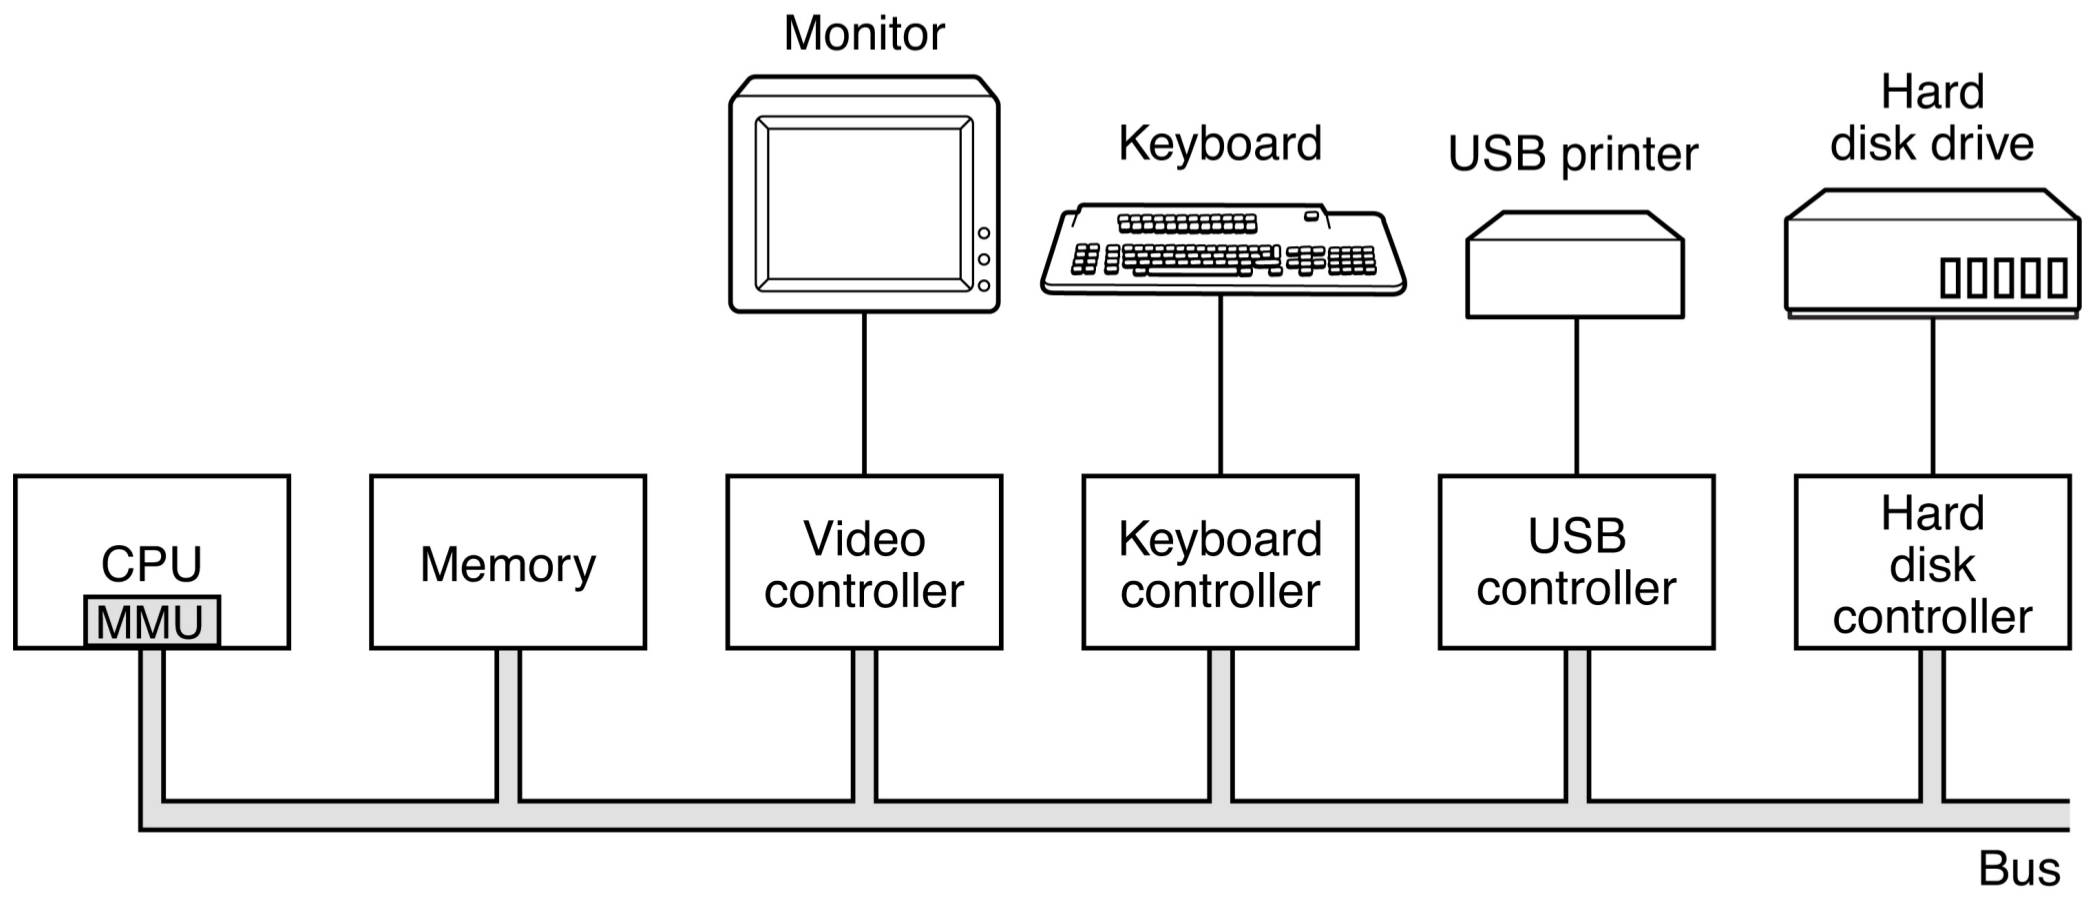
\includegraphics[width=0.33\textwidth]{BusSystem}\end{figure}
	\item today: multiple busses
	\begin{figure}[H]\centering\label{BusSystemToday}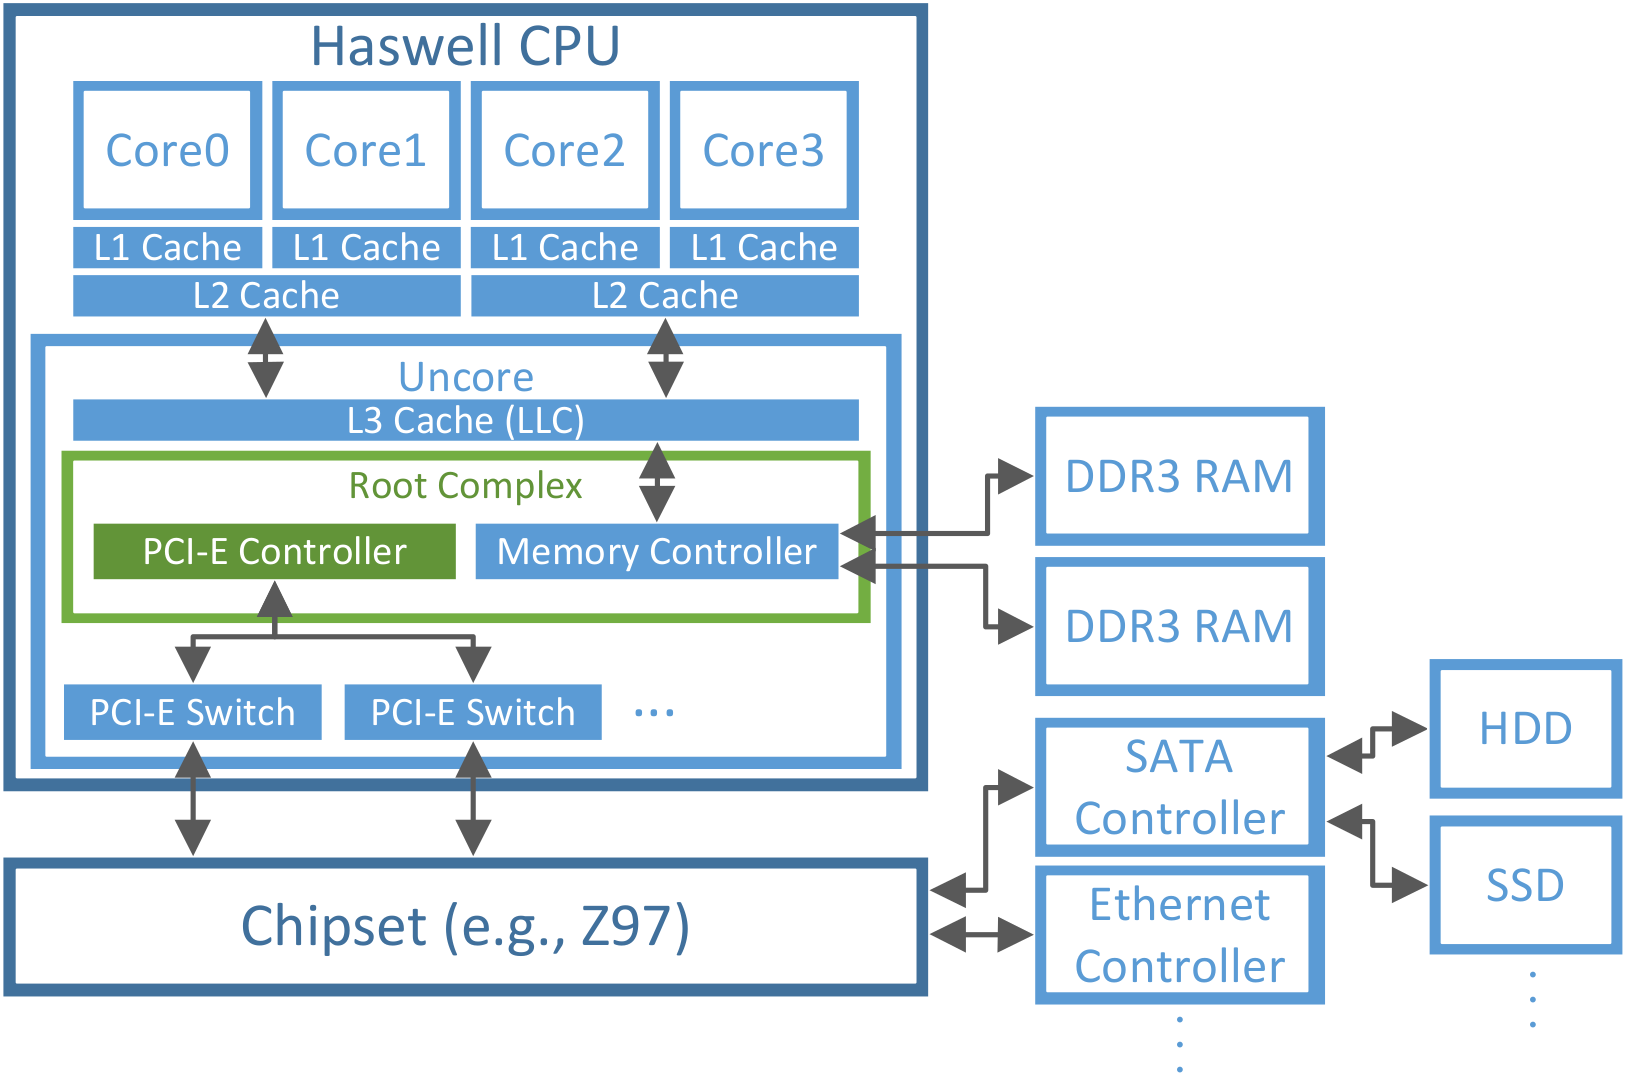
\includegraphics[width=0.33\textwidth]{BusSystemToday}\end{figure}
\end{items}

\textbf{Central Processing Unit (CPU) -- Operation}
\begin{items}
	\item fetches instructions from memory, executes them (instruction format/-set depends on CPU)
	\item CPU internal registers store (meta-)data during execution (general purpose registers, floating point registers, instruction pointer (IP), stack pointer (SP), program status word (PSW),...)
	\item \underline{execution modes}: \\*
		\textbf{user mode} (x86: \emph{Ring 3}/\emph{CPL 3}): \\*
			\phantom{x} only non-privileged instructions may be executed \\*
			\phantom{x} cannot manage hardware \( \to \) \textbf{protection} \\*
		\textbf{kernel mode} (x86: \emph{Ring 0}/\emph{CPL 0}): \\*
			\phantom{x} all instructions allowed \\*
			\phantom{x} can manage hw with \textbf{privileged instructions}
		\begin{figure}[H]\centering\label{OperationModes}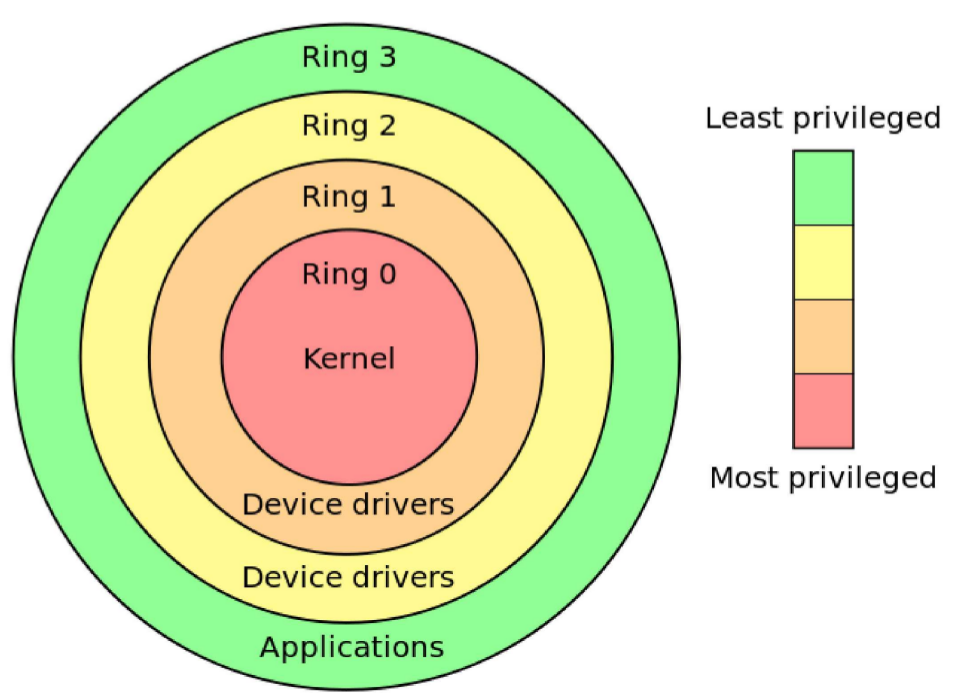
\includegraphics[width=0.2\textwidth]{OperationModes}\end{figure}
\end{items}

\textbf{Random Access Memory (RAM)}
\begin{items}
	\item keeps currently executed instructions + data
	\item today: CPUs have built-in \emph{memory controller}
	\item root complex connected directly via \\*
		"`wire"' to caches \\*
		pins to RAM \\*
		pins to PCI-E switches
\end{items}

\textbf{Caching}
\begin{items}
	\item RAM delivers instructions/data slower than CPU can execute
	\item memory references typicalle follow \emph{locality principle}: \\*
		\textbf{spatial locality}: future refs often near previous accesses \\*
			\phantom{x} (e.g. next byte in array) \\*
		\textbf{temporal locality}: future refs often at previously accessed ref \\*
			\phantom{x} (e.g. loop counter)
	\item \emph{caching} helps mitigating this memory wall: \\*
		copy used information temporarily from slower to faster storage \\*
		check faster storage first before going down \textbf{memory hierarchy} \\*
		if not, data is copied to cache and used from there
	\item \underline{Access latency}: \\*
		register: \( \sim \)1 CPU cycle \\*
		L1 cache (per core): \( \sim \)4 CPU cycles \\*
		L2 cache (per core pair): \( \sim \)12 CPU cycles \\*
		L3 cache/LLC (per uncore): \( \sim \)28 CPU cycles (\( \sim \)25 GiB/s) \\*
		DDR3-12800U RAM: \( \sim \)28 CPU cycles + \( \sim \) 50ns (\( \sim \)12 GiB/s)
\end{items}

\textbf{Caching -- Cache Organisation}
\begin{items}
	\item caches managed in hardware
	\item divided into \emph{cache lines} (usually 64 bytes each, unit at which data is exchanged between hierarchy levels)
	\item often separation of data/instructions in faster caches (e.g. L1, see \emph{harward architecture})
	\item \textbf{cache hit}: accessed data already in cache (e.g. L2 cache hit)
	\item \textbf{cache miss}: accessed data has to be fetched from lower level
	\item cache miss types: \\*
		\emph{compulsory miss}: first ref miss, data never been accessed \\*
		\emph{capacity miss}: cache not large enough for process working set \\*
		\emph{conflict miss}: cache has still space, but collisions due to \\* \phantom{x} placement strategy
\end{items}

\textbf{Interplay of CPU and Devices}
\begin{items}
	\item I/O devices and CPU execute concurrently
	\item Each device controller \\*
		- is in charge of particular device \\*
		- has local buffer
	\item \underline{Workflow}:
	\begin{enumeration}
		\item CPU issues commands, moves data to devices
		\item Device controller informs APIC that operation is finished
		\item APIC signals CPU
		\item CPU receives device/interrupt number from APIC, executes handler
	\end{enumeration}
	\begin{figure}[H]\centering\label{CPUIOInterplay}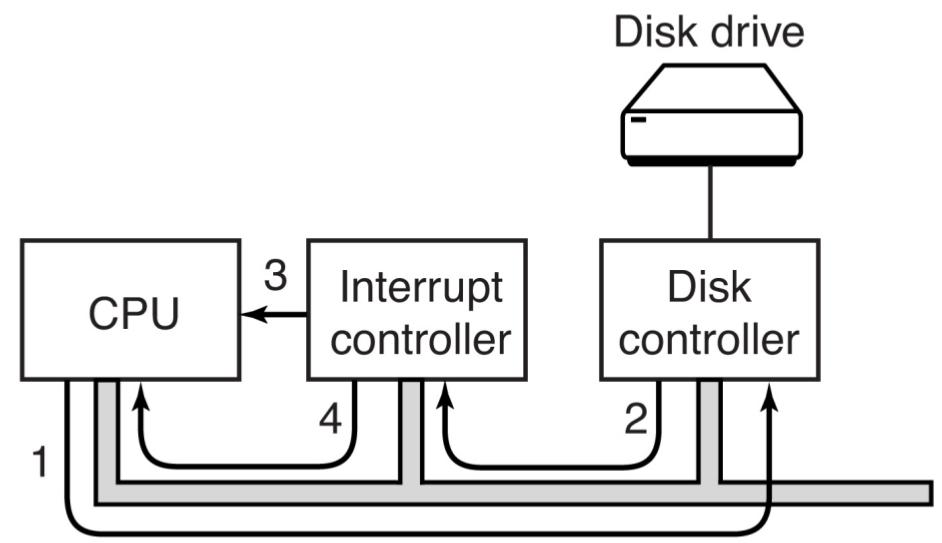
\includegraphics[width=0.2\textwidth]{CPUIOInterplay}\end{figure}
\end{items}

\newpage 

\textbf{Device control}
\begin{items}
	\item Devices controlled through their \textbf{device controller}, accepts commands from OS via \textbf{device driver}
	\item devices controlled through device registers and device memory: \\*
		\emph{control} device by writing device registers \\*
		\emph{read} status of device by reading device registers \\*
		\emph{pass data} to device by reading/writing device memory
	\item 2 ways to access device registers/memory:
	\begin{enumeration}
		\item \textbf{port-mapped IO} (PMIO): \\*
			use special CPU instructions to access port-mapped \\* \phantom{x} registers/memory \\*
			e.g. x86 has different \code{in}/\code{out}-commands that transfer \\* \phantom{x} 1,2 or 4 bytes between CPU and device
		\item \textbf{memory-mapped IO} (MMIO): \\*
			use same address space for RAM and device memory \\*
			some addresses map to RAM, others to different devices \\*
			access device's memory region to access device registers/memory
	\end{enumeration}
	\item some devices use hybrid approaches using both
\end{items}

\textbf{Device control -- Nvidia general purpose GPU}
\begin{items}
	\item memory-mapped ring-buffer and \code{put}/\code{get}-device
	\item mapping can be exposed to application \( \leadsto \) application can submit commands in user-mode
	\begin{figure}[H]\centering\label{NvidiaRing}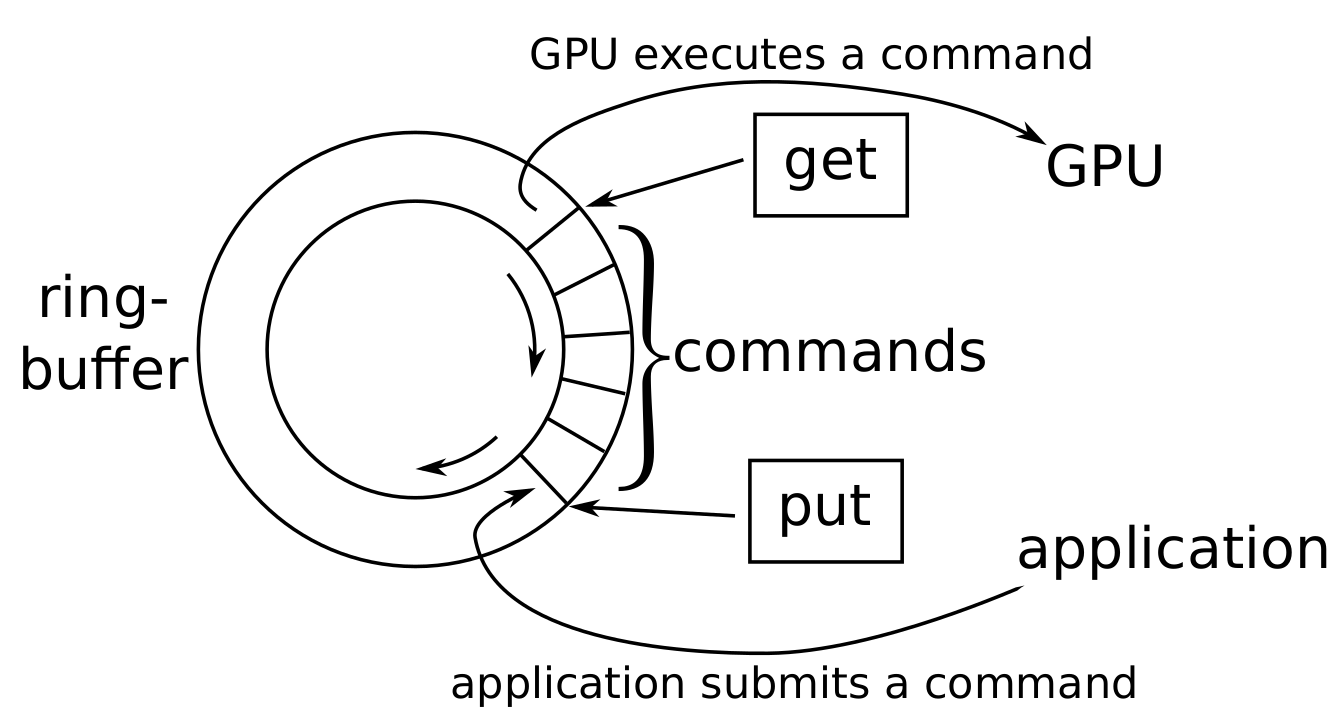
\includegraphics[width=0.33\textwidth]{NvidiaRing}\end{figure}
\end{items}

\begin{summary}
	\begin{items}
		\setlength\itemsep{0em}
		\item The OS is an abstraction layer between applications and hardware (multiplexes hardware, hides hardware details, provides protextion between processes/users)
		\item The CPU provides a separation of User and Kernel mode (which are required for an OS to provide protection between applications)
		\item CPU can execute commands faster than memore can deliver instructions/data -- memory hierarchy mitigates this memory wall, needs to be carefully managed by OS to minimize slowdowns
		\item device drivers control hardware devices through PMIO/MMIO
		\item Devices can signal the CPU (and through the CPU notify the OS) through interrupts
	\end{items}
\end{summary}

  % \newpage

  % \section{OS Concepts}

\paragraph{OS Invocation}
\begin{itemize}
	\item OS Kernel does \textbf{not} always run in background!
	\item Occasions invoking kernel, switching to kernel mode:
	\begin{enumerate}
		\item \textbf{System calls}: User-Mode processes require higher privileges
		\item \textbf{Interrupts}: CPU-external device sends signal
		\item \textbf{Exceptions}: CPU signals unexpected condition
	\end{enumerate}
\end{itemize}

\paragraph{System Calls --- Motivation}
\begin{itemize}
	\item \textbf{Problem}: protect processes from one another
	\item \textbf{Idea}: Restrict processes by running them in user-mode
	\item \textbf{$ \leadsto $ Problem}: now processes cannot manage hardware,...
	\begin{itemize}
		\item who can switch between processes?
		\item who decides if process may open certain file?
	\end{itemize}
	\item \textbf{$ \leadsto $ Idea}: OS provides \textbf{services} to apps
	\begin{enumerate}
		\item app calls system if service is needed (\textbf{syscall})
		\item OS checks if app is allowed to perform action
		\item if app may perform action and hasn't exceeded quota, OS performs action in behalf of app in kernel mode
	\end{enumerate}
\end{itemize}

\paragraph{System Calls --- Examples}
\begin{itemize}
	\item \code{fd = open(file, how,...)} -- open file for read/write/both
	\item documented e.g. in \code{man 2 write}
	\item overview in \code{man 2 syscalls}
\end{itemize}

\paragraph{System Calls vs. APIs}
\begin{itemize}
	\item \textbf{Syscalls}: interface between apps and OS services, limited number of well-defined entry points to kernel
	\item \textbf{APIs}: often used by programmers to make syscalls (e.g. \code{printf} library call uses \code{write} syscall)
	\item common APIs: Win32, POSIX, C API
\end{itemize}

\paragraph{System Calls --- Implementation}
\begin{itemize}
	\item \textbf{Trap Instruction}: single syscall interface (entry point) to kernel
	\begin{itemize}
		\item switches CPU to kernel mode, enters kernel in same way for all syscalls
		\item \emph{system call dispatcher} in kernel then acts as syscall multiplexer
	\end{itemize}
	\item \textbf{Syscall Identification}: number passed to trap instruction
	\begin{itemize}
		\item \emph{Syscall Table} maps syscall numbers to kernel functions
		\item \emph{Dispatcher} decides where to jump based on number and table
		\item programs (e.g. \code{stdlib}) have syscall number compiled in!
	\end{itemize}
	$ \leadsto $ never reuse old syscall numbers in future kernel versions
\end{itemize}

\paragraph{Interrupts}
\begin{itemize}
	\item \textbf{Devices}: use interrupts to signal predefined conditions to OS
	\begin{itemize}
		\item \emph{reminder}: device has ``interrupt line'' to CPU (e.g. device controller informs CPU that operation is finished)
	\end{itemize}
	\item \textbf{Programmable Interrupt Controller}: manages interrupts
	\begin{itemize}
		\item interrupts can be \emph{masked} (queued, delivered when interrupt unmasked)
		\item queue has finite length $ \leadsto $ interrupts can get lost
	\end{itemize}
	\item \textbf{Examples}:
	\begin{enumerate}
		\item \emph{timer-interrupt}: periodically interrupts processes, switches to kernel $ \leadsto $ can then switch to different processes for fairness
		\item \emph{network interface card} interrupts CPU when packet was received $ \leadsto $ can deliver packet to process and free NIC buffer
	\end{enumerate}
	\item \textbf{Interrupt process}:
	\begin{enumerate}
		\item CPU looks up \emph{interrupt vector} (= table pinned in memory, contains addresses of all service routines)
		\item CPU transfers control to respective \emph{interrupt service routine} in OS that handles interrupt
	\end{enumerate}
	$ \leadsto $ interrupt service routine must first save interrupted process's state (instruction pointer, stack pointer, status word)
\end{itemize}

\paragraph{Exceptions}
\begin{itemize}
	\item \textbf{Motivation}: unusual condition $ \to $ impossible for CPU to continue processing
	\item $ \leadsto $ \textbf{Exception} generated within CPU:
	\begin{enumerate}
		\item CPU interrupts program, gives kernel control
		\item kernel determines reason for exception
		\item if kernel can resolve problem $ \leadsto $ does so, continues \emph{faulting instruction}
		\item kills process if not
	\end{enumerate}
	\item \textbf{Difference to Interrupts}: interrupts can happen in any context, exceptions always occur asynchronous and in process context
\end{itemize}

\paragraph{OS Concepts --- Physical Memory}
\begin{itemize}
	\item up to early 60s:
	\begin{itemize}
		\item programs loaded and run directly in \emph{physical memory}
		\item program too large $ \to $ partitioned manually into \emph{overlays}
		\item OS: swaps overlays between disk and memory
		\item different jobs could observe/modify each other
	\end{itemize}
\end{itemize}

\paragraph{OS Concepts --- Address Spaces}
\begin{itemize}
	\item \textbf{Motivation}: bad programs/people need to be isolated
	\item \textbf{Idea}: give every job the illusion of having all memory to itself
	\begin{itemize}
		\item every job has own \emph{address space}, can't name addresses of others
		\item jobs always and only use virtual addresses
	\end{itemize}
\end{itemize}

\paragraph{Virtual Memory --- Indirect Addressing}
\begin{itemize}
	\item \textbf{MMU}: every CPU has built-in \emph{memory management unit} (MMU)
	\item \textbf{Principle}: translates virtual addresses to physical addresses at every load/store \\
	$ \leadsto $ address translation protects one program from another
	\item \textbf{Definitions}:
	\begin{itemize}
		\item \emph{Virtual address}: address in process' address space
		\item \emph{Physical address}: address of real memory
	\end{itemize}
\end{itemize}

\paragraph{Virtual Memory --- Memory Protection}
\begin{itemize}
	\item \textbf{Kernel-only Virtual Addresses}
	\begin{itemize}
		\item kernel typically part of all address spaces
		\item ensures that apps can't touch kernel memory
	\end{itemize}
	\item \textbf{Read-only virtual addresses}: can be enforced by MMU
	\begin{itemize}
		\item allows safe sharing of memory between apps
	\end{itemize}
	\item \textbf{Execute Disable}: can be enforced by MMU
	\begin{itemize}
		\item makes code injection attacks harder
	\end{itemize}
\end{itemize}

\paragraph{Virtual Memory --- Page Faults}
\begin{itemize}
	\item \textbf{Motivation}: not all addresses need to be mapped at all times
	\begin{itemize}
		\item MMU issues \emph{page fault} exception when accessed virtual address isn't mapped
		\item OS handles page faults by loading faulting addresses and then continuing the program
		\item[$ \leadsto $] memory can be \emph{over-committed}: more memory than physically available can be allocated to application
	\end{itemize}
	\item \textbf{Illegal addresses}: page faults also issued by MMU on illegal memory accesses
\end{itemize}

\paragraph{OS Concepts --- Processes}
\begin{itemize}
	\item \textbf{Process}: program in execution (``instance'' of program)
	\item each process is associated with
	\begin{itemize}
		\item \textbf{Process Control Block} (PCB): contains information about allocated resources
		\item virtual \textbf{Address Space} (AS):
		\begin{itemize}
			\item all (virtual) memory locations a program can name
			\item starts at 0 and runs up to a maximum
			\item address 123 in AS1 generally $ \neq $ address 123 in AS2
			\item indirect addressing $ \leadsto $ different ASes to different programs
			\item[$ \leadsto $] \emph{protection between processes}
		\end{itemize}
	\end{itemize}
\end{itemize}

\paragraph{OS Concepts --- Address Space Layout}
\begin{itemize}
	\item \textbf{Sections}: address spaces typically laid-out in different sections
	\begin{itemize}
		\item memory addresses between sections \emph{illegal}
		\item illegal addresses $ \leadsto $ page fault (\emph{segmentation fault})
		\item OS usually kills process causing segmentation fault
	\end{itemize}
	\item \textbf{Important sections}:
	\begin{itemize}
		\item \emph{Stack}: function history, local variables
		\item \emph{Data}: Constants, static/global variables, strings
		\item \emph{Text}: Program code
	\end{itemize}
\end{itemize}
\begin{figure}[h]\centering\label{AddressSpaceLayout}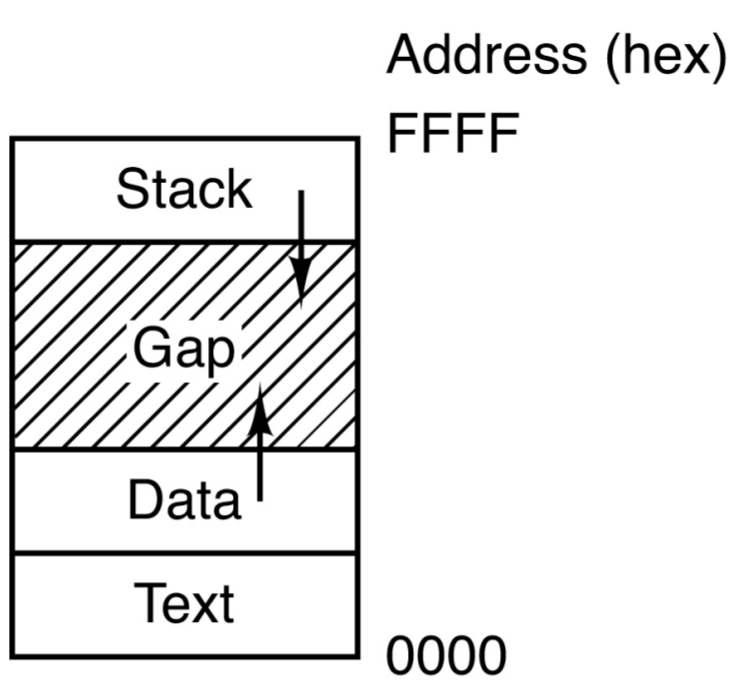
\includegraphics[width=0.15\textwidth]{AddressSpaceLayout}\end{figure}

\paragraph{OS Concepts --- Threads}
\begin{itemize}
	\item \textbf{Thread}: represents execution state of process ($ \geq 1 $ thread per process)
	\begin{itemize}
		\item \emph{IP}: stores currently executed instruction (address in \code{text} section)
		\item \emph{SP}: stores address of stack top ($ > 1 $ threads $ \to $ multiple stacks!)
		\item \emph{PSW}: contains flags about execution history (e.g. last calculation was 0 $ \to $ used in following jump instruction)
		\item more general purpose registers, floating point registers,...
	\end{itemize}
\end{itemize}
\begin{figure}[h]\centering\label{Threads}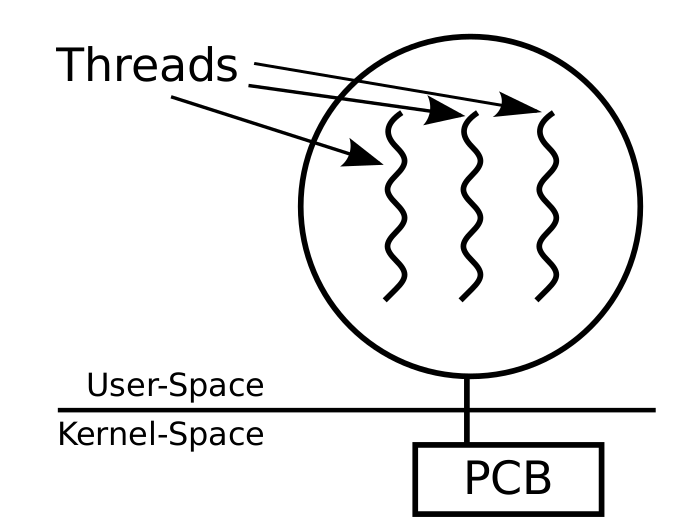
\includegraphics[width=0.2\textwidth]{Threads}\end{figure}

\paragraph{OS Concepts --- Policies vs. Mechanisms}
\begin{itemize}
	\item \textbf{Mechanism}: implementation of what is done (e.g. commands to write to HDD)
	\item \textbf{Policy}: rules which decide when what is done and how much (e.g. how often, how many resources are used,...)
	\item[$ \to $] \emph{mechanisms can be reused even when policy changes}
\end{itemize}

\paragraph{OS Concepts --- Scheduling}
\begin{itemize}
	\item \textbf{Motivation}: multiple processes/threads available $ \leadsto $ OS needs to switch between them (for multitasking)
	\item \textbf{Scheduler}: decides which job to run next (\emph{policy}) --- tries to
	\begin{itemize}
		\item provide fairness
		\item meet performance goals
		\item adhere to priorities 
	\end{itemize}
	\item \textbf{Dispatcher}: performs task-switching (\emph{mechanism})
\end{itemize}
\begin{figure}[h]\centering\label{Scheduling}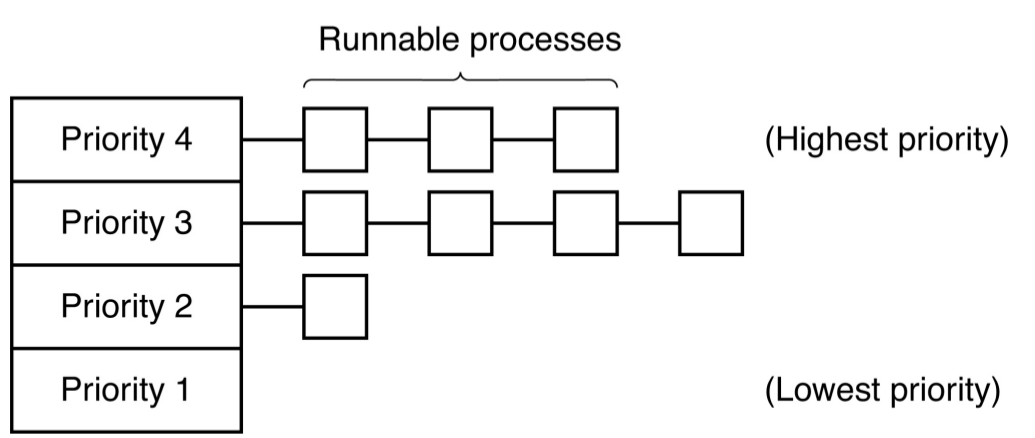
\includegraphics[width=0.33\textwidth]{Scheduling}\end{figure}

\paragraph{OS Concepts --- Files}
\begin{itemize}
	\item \textbf{Motivation}: OS hides peculiarities of file storage, programmer uses device-independent \emph{files}/\emph{directories}
	\item \textbf{Files}: associate \emph{file name} and \emph{offset} with bytes
	\item \textbf{Directories}: associate \emph{directory names} with directory names or file names
	\item \textbf{File System}: ordered block collection
	\begin{itemize}
		\item main task: translate (dir name + file name + offset) to block
		\item programmer uses file system operations to operate on files (\code{open}, \code{read}, \code{seek})
		\item processes can communicate directly through special \emph{named pipe} file (used with same operations as any other file)
	\end{itemize}
\end{itemize}

\paragraph{OS Concepts --- Directory Tree}
\begin{itemize}
	\item \textbf{Directories}: form \emph{directory tree}/\emph{file hierarchy}
		$ \to $ structure data
	\item \textbf{Root Directory}: topmost directory in tree
	\item \textbf{Path Name}: used to specify file
\end{itemize}

\paragraph{OS Concepts --- Mounting}
\begin{itemize}
	\item \textbf{Unix}: common to orchestrate multiple file systems in single file hierarchy
	\item file systems can be \emph{mounted} on directory
	\item \textbf{Win}: manage multiple directory hierarchies with drive letters (e.g. \code{C:\\Users})
\end{itemize}

\paragraph{OS Concepts --- Storage Management}
\begin{itemize}
	\item \textbf{OS}: provides uniform view of information storage to file systems
	\begin{itemize}
		\item \emph{Drivers}: hide specific hardware devices $ \to $ hides device peculiarities
		\item general interface abstracts physical properties to logical units $ \to $ block
	\end{itemize}
	\item \textbf{Performance}: OS increases I/O performance:
	\begin{itemize}
		\item \emph{Buffering}: Store data temporarily while transferred
		\item \emph{Caching}: Store data parts in faster storage
		\item \emph{Spooling}: Overlap one job's output with other job's input
	\end{itemize}
\end{itemize}

\begin{summary}
	\begin{itemize}
		\item \textbf{OS}: provides abstractions for and protection between applications
		\item \textbf{Kernel}: does not always run --- certain events invoke kernel
		\begin{itemize}
			\item \emph{syscall}: process asks kernel for service
			\item \emph{interrupt}: device sends signal that OS has to handle
			\item \emph{exception}: CPU encounters unusual situation
		\end{itemize}
		\item \textbf{Processes}: encapsulate resources needed to run program in OS
		\begin{itemize}
			\item \emph{threads}: represent different execution states of process
			\item \emph{address space}: all memory process can name
			\item \emph{resources}: allocated resources, e.g., open files
		\end{itemize}
		\item \textbf{Scheduler} decides which process to run next when multi-tasking
		\item \textbf{Virtual Memory} implements address spaces, provides protection between processes
		\item \textbf{File system} abstracts background store using I/O drivers, provides simple interface (files + directories)
	\end{itemize}
\end{summary}

  % \section{Processes}

\paragraph{The Process Abstraction}
\begin{itemize}
	\item computers do "`several things at the same time"' (just looks this way though quick process switching (\textbf{Multiprogramming}))
	\item \( \leadsto \) \textbf{process} abstraction models this concurrency: \\*
		- container contains information about program execution \\*
		- conceptually, every progress has own "`virtual CPU"' \\*
		- execution context is changed on process switch \\*
		- dispatcher switches context when switching processes \\*
		- \textbf{context switch}: dispatcher saves current registers/memory \\* \phantom{-} mappings, restores those of next process
\end{itemize}

\paragraph{Process-Cooking Analogy}
\begin{itemize}
	\item Program/Process like Recipe/Cooking
	\item \textbf{Recipe}: lists ingredients, gives algorithm what to do when \\*
		\( \leadsto \) program describes memory layout/CPU instructions
	\item \textbf{Cooking}: activity of using the recipe \\*
		\( \leadsto \) process is activity of executing a program
	\item multiple similar recipes for same dish \\*
		\( \leadsto \) multiple programs may solve same problem
	\item recipe can be cooked in different kitchens at the same time \\*
		\( \leadsto \) program can be run on different CPUs at the same time \\* \phantom{\( \leadsto \)} (as different processes)
	\item multiple people can cook one recipe \\*
		\( \leadsto \) one process can have several worker threads
\end{itemize}

\paragraph{Concurrency vs. Parallelism}
\begin{itemize}
	\item OS uses currency + parallelism to implement multiprogramming
	\begin{enumerate}
		\item \textbf{Concurrency}: multiple processes, one CPU \\* \( \leadsto \) not at the same time
		\item \textbf{Parallelism}: multiple processes, multiple CPU \\* \( \leadsto \) at the same time
	\end{enumerate}
\end{itemize}

\paragraph{Virtual Memory Abstraction --- Address Spaces}
\begin{itemize}
	\item every process has own \emph{virtual addresses} (vaddr)
	\item MMU relocates each load/store to \emph{physical memory} (pmem)
	\item processes never see physical memory, can't access it directly
	\item \textcolor{black!60!green}{\code{+}} MMU can enforce protection (mappings in kernel mode)
	\item \textcolor{black!60!green}{\code{+}} programs can see more memory than available \\*
		\phantom{x} 80:20 rule: 80\% of process memory idle, 20\% active \\*
		\phantom{x} can keep working set in RAM, rest on disk
	\item \textcolor{red}{\code{-}} need special MMU hardware
\end{itemize}

\paragraph{Address Space (Process View)}
\begin{itemize}
	\item code/data/state need to be organized within process \\*
		\( \leadsto \) \textbf{address space layout}
	\item Data types:
	\begin{enumerate}
		\item \emph{fixed size} data items
		\item data naturally \emph{freed in reverse allocation order}
		\item data \emph{allocated/freed "`randomly"'}
	\end{enumerate}
	\item compiler/architecture determine how large int is and what instructions are used in text section (\code{code})
	\item \textbf{Loader} determines based on exe file how executed program is placed in memory
\end{itemize}

\paragraph{Segments --- Fixed-Size Data + Code}
\begin{itemize}
	\item some data in programs never changes or will be written but never grows/shrinks \\*
		\( \leadsto \) memory can be statically allocated on process creation
	\item \textbf{BSS segment} (\emph{block started by symbol}): \\*
		- statically allocated variables/non-initialized variables \\*
		- executable file typically contains starting address + size of BSS \\*
		- entire segment initially 0
	\item \textbf{Data segment}: \\*
		- fixed-size, initialized data elements (e.g. global variables)
	\item \textbf{read-only data segment}: \\*
		- constant numbers, strings
	\item All three sometimes summarized as one segment
	\item compiler and OS decide ultimately where to place which data/how many segments exist
\end{itemize}

\paragraph{Segments --- Stack}
\begin{itemize}
	\item some data naturally freed in reverse allocation order \\*
		\( \leadsto \) very easy memory management (stack grows upwards)
	\item fixed segment starting point
	\item store top of latest allocation in \textbf{stack pointer} (SP) \\*
		(initialized to starting point)
	\item \emph{allocate} \code{a} byte data structure: \code{SP += a; return(SP - a)}
	\item \emph{free} \code{a} byte data structure: \code{SP -= a}
\end{itemize}

\paragraph{Segments --- Heap (Dynamic Memory Allocation)}
\begin{itemize}
	\item some data "`randomly"' allocated/freed
	\item two-tier memory allocation:
	\begin{enumerate}
		\item allocate large memory chunk (\textbf{heap segment}) from OS \\*
			- base address + \textbf{break pointer} (BRK) \\*
			- process can get more/give back memory from/to OS \\*
		\item dynamically partition chunk into smaller allocations \\*
			- \code{malloc}/\code{free} can be used in random oder \\*
			- purely user-space, no need to contact kernel
	\end{enumerate}
\end{itemize}

\begin{figure}[h]\centering\label{AddressSpaceLayoutComplex}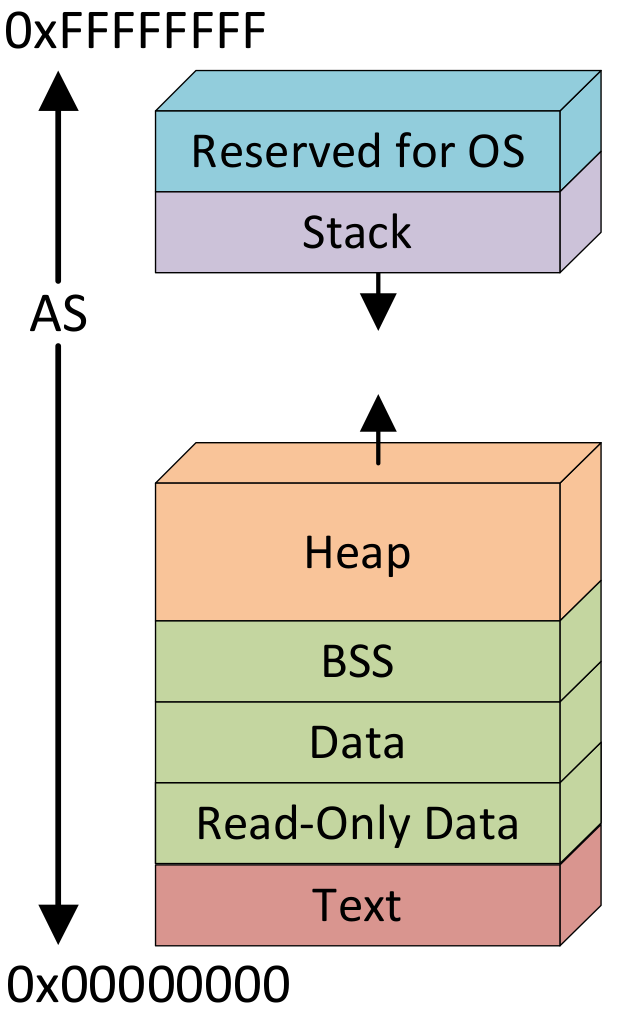
\includegraphics[width=0.2\textwidth]{AddressSpaceLayoutComplex}\end{figure}

\begin{summary}
	\begin{itemize}
		\item recipe vs. cooking is like program vs. process
		\item processes = resource container for OS
		\item process feels alone: has own CPU + memory
		\item OS implements multiprogramming through rapid process switching
	\end{itemize}
\end{summary}

  % \section{Process API}

\textbf{Execution Model -- Assembler (simplified)}
\begin{items}
  \item OS interacts directly with compiled programs \\*
    - switch between processes/threads \( \leadsto \) \textbf{save}/\textbf{restore} state \\*
    - deal with/pass on \textbf{signals}/\textbf{exceptions} \\*
    - receive \textbf{requests} from applications
  \item \underline{Instructions}: \\*
    - \code{mov}: Copy referenced data from second operand to first operand \\*
    - \code{add}/\code{sub}/\code{mul}/\code{div}: Add,\dots from second operand to first operand \\*
    - \code{inc}/\code{dec}: increment/decrement register/memory location \\*
    - \code{shl}/\code{shr}: shift first operand left/right by amount given by second operand \\*
    - \code{and}/\code{or}/\code{xor}: calculate bitwise and,\dots of two operands storing result in first \\*
    - \code{not}: bitwise negate operand
\end{items}

\ \\
\textbf{Execution Model -- Stack (x86)}
\begin{items}
  \item \underline{stack pointer} (SP): holds address of stack top (growing downwards)
  \item \underline{stack frames}: larger stack chunks
  \item \underline{base pointer} (BP): used to organize stack frames
\end{items}

\ \\
\textbf{Execution Model -- jump/branch/call commands (x86)}
\begin{items}
  \item \code{jmp}: continue execution at operand address
  \item \code{j\$condition}: jump depending on PSW content \\*
    true \( \leadsto \) jump \\*
    false \( \leadsto \) continue \\*
    examples: \code{je} (jump equal), \code{jz} (jump zero)
  \item \code{call}: push function to stack and jump to it
  \item \code{return}: return from function (jump to return address)
\end{items}

\ \\
\textbf{Execution Model -- Application Binary Interface (ABI)}
\begin{items}
  \item standardizes binary interface between programs, modules, OS: \\*
    - executable/object file layout \\*
    - calling conventions \\*
    - alignment rules
  \item \underline{calling conventions}: standardize exact way function calls are implemented \\*
    \( \leadsto \) interoperability between compilers
\end{items}

\textbf{Execution Model -- calling conventions (x86)}
\begin{items}
  \item function call (caller):
  \begin{enumeration}
    \item save local scope state 
    \item set up parameters where function can find them
    \item transfer control flow
  \end{enumeration}
  \item function call (called function):
  \begin{enumeration}
    \item set up new local scope (local variables)
    \item perform duty
    \item put return value where caller can find it
    \item jump back to caller (IP)
  \end{enumeration}
\end{items}

  % \section{Threads}

\paragraph{Processes vs. Threads}
\begin{itemize}
  \item \textbf{Traditional OS}: each process has
  \begin{itemize}
    \item own address space
    \item own set of allocated resources
    \item \emph{one} thread of execution ( = one execution state)
  \end{itemize}
  \item \textbf{Modern OS}: processes + threads of execution handled more flexibly
  \begin{itemize}
    \item \emph{processes} provide abstraction of address space and resources
    \item \emph{threads} provide abstraction of execution states of that address space
  \end{itemize}
  \item \textbf{Exceptions}:
  \begin{itemize}
    \item sometimes different threads have different address spaces
    \item \emph{Linux}: threads = regular processes with shared resources and AS regions
  \end{itemize}
\end{itemize}

\paragraph{Threads --- why?}
\begin{itemize}
  \item many programs do multiple things at once (e.g. web server)
  \begin{itemize}
    \item[$ \leadsto $] writing program as many sequential threads may be easier than with blocking operations
  \end{itemize}
  \item \textbf{Processes}: rarely share data (if, then explicitly)
  \item \textbf{Threads}: closely related, share data
\end{itemize}
\begin{figure}[h]\centering\label{ProcessesThreads}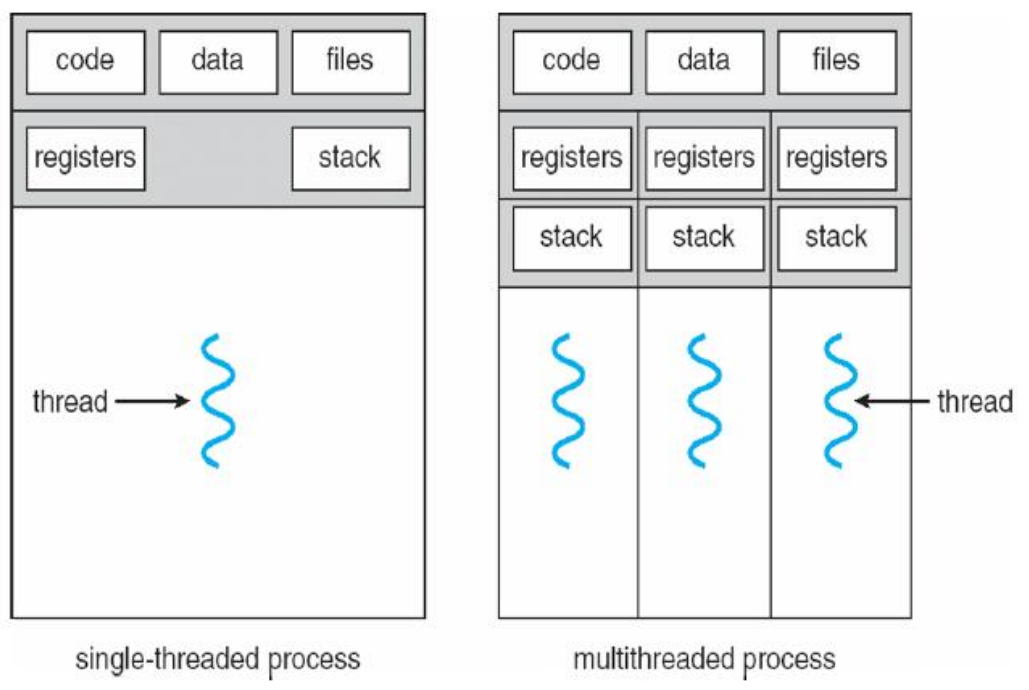
\includegraphics[width=0.33\textwidth]{ProcessesThreads}\end{figure}

\paragraph{Threads --- POSIX}
\begin{itemize}
  \item \code{Pthread}: base object with
  \begin{itemize}
    \item \emph{identifier} (thread ID, TID)
    \item \emph{register set} (including IP and SP)
    \item \emph{stack area} to hold execution state
  \end{itemize}
  \item \code{pthread_create}: create new thread
  \begin{itemize}
    \item Pass: \emph{pointer} to \code{pthread_t} (will hold TID after successful call)
    \item Pass: \emph{attributes}, \emph{start function}, \emph{arguments}
    \item Returns: \code{0} on success, error value else
  \end{itemize}
  \item \code{pthread_exit}: terminate calling thread
  \begin{itemize}
    \item Pass: exit code (casted to void pointer)
    \item Free's resources (e.g. stack)
  \end{itemize}
  \item \code{pthread_join}: wait for specified thread to exit
  \begin{itemize}
    \item Pass: \code{ptread_t} to wait for (or \code{-1} for any thread)
    \item Pass: pointer to pointer for exit code
    \item Returns: \code{0} on success, error value else
  \end{itemize}
  \item \code{pthread_yield}: release CPU to let another thread run
\end{itemize}

\paragraph{Threads --- Problems}
\begin{itemize}
  \item \textbf{Processes vs. Threads}:
  \begin{itemize}
    \item \emph{Processes}: only share resources explicitly
    \item \emph{Threads}: more shared state \( \to \) more can go wrong
  \end{itemize}
  \item \textbf{Challenges}: programmer needs to take care of
  \begin{itemize}
    \item \emph{activities}: dividing, ordering, balancing
    \item \emph{data}: dividing
    \item \emph{shared data}: access synchronizing
  \end{itemize}
\end{itemize}

\paragraph{PCB vs. TCB}
\begin{itemize}
  \item \textbf{PCB} (\emph{process control block}): information needed to implement processes
  \begin{itemize}
    \item always known to OS
  \end{itemize}
  \item \textbf{TCB} (\emph{thread control block}): per thread data
  \begin{itemize}
    \item OS knowledge depends on \emph{thread model}
  \end{itemize}
\end{itemize}
\begin{figure}[H]\centering\label{PCBTCB}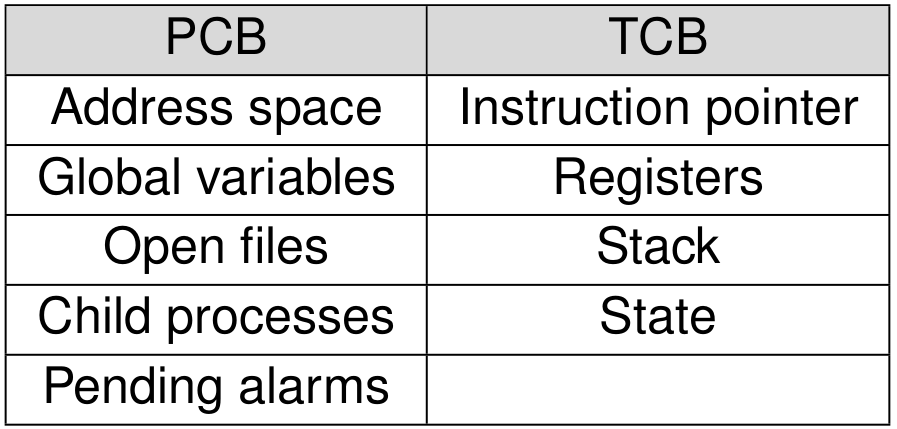
\includegraphics[width=0.2\textwidth]{PCBTCB}\end{figure}

\paragraph{Thread models}
\begin{itemize}
  \item \textbf{Kernel Thread}: known to OS kernel
  \item \textbf{User Thread}: known to process
  \item \textbf{N:1-Model}: kernel only knows one of possibly multiple threads
  \begin{itemize}
    \item N:1 user threads = \emph{user level threads} (ULT)
  \end{itemize}
  \item \textbf{1:1-Model}: each user thread maps to one kernel thread
  \begin{itemize}
    \item 1:1 user threads = \emph{kernel level threads} (KLT)
  \end{itemize}
  \item \textbf{M:N-Model} (hybrid model): flexible mapping of user threads to fewer kernel threads 
\end{itemize}

\paragraph{Thread models --- N:1}
\begin{itemize}
  \item Kernel only manages process \( \to \) multiple threads unknown to kernel 
  \item Threads managed in user-space library (e.g. GNU Portable Threads)
  \item \textbf{Pro}:
  \begin{itemize}
    \item[+] faster thread management operations (up to 100 times)
    \item[+] flexible scheduling policy
    \item[+] few system resources
    \item[+] usable even if OS doesn't support threads
  \end{itemize}
  \item \textbf{Con}:
  \begin{itemize}
    \item[-] no parallel execution
    \item[-] whole process blocks if one user thread blocks
    \item[-] reimplementing OS parts (e.g. scheduler)
  \end{itemize}
  \item \textbf{Stack}:
  \begin{itemize}
    \item main stack known to OS used by thread library
    \item own execution state (= stack) dynamically allocated by user thread library for each thread
    \item possibly own stack for each exception handler
  \end{itemize}
  \item \textbf{Heap}:
  \begin{itemize}
    \item concurrent heap use possible
    \item \emph{Attention}: not all heaps are reentrant
  \end{itemize}
  \item \textbf{Data}: divided into BSS, data and read-only data here as well
\end{itemize}
\begin{figure}[h]\centering\label{ULTAddressSpace}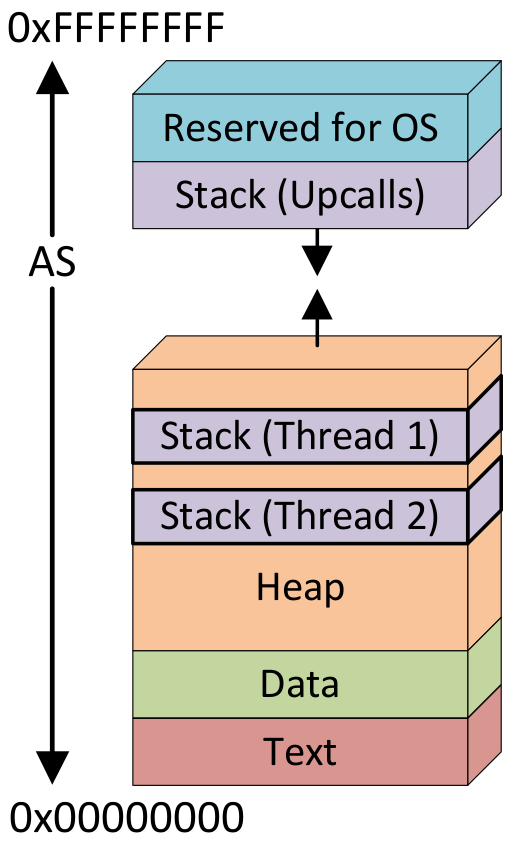
\includegraphics[width=0.15\textwidth]{ULTAddressSpace}\end{figure}

\paragraph{Thread models --- 1:1}
\begin{itemize}
  \item kernel knows + manages every thread
  \item \textbf{Pros}:
  \begin{itemize}
    \item[+] real parallelism possible
    \item[+] threads block individually
  \end{itemize}
  \item \textbf{Cons}:
  \begin{itemize}
    \item[-] OS manages every thread in system (TCB, stacks,\dots)
    \item[-] Syscalls needed for thread management
    \item[-] scheduling fixed in OS
  \end{itemize}
  \item \textbf{Stack}:
  \begin{itemize}
    \item own execution state (= stack) for every thread
    \item possibly own stack for (each) exception handler
  \end{itemize}
  \item \textbf{Heap}:
  \begin{itemize}
    \item parallel heap use possible
    \item \emph{Attention}: not all heaps are thread-safe
    \item if thread-safe: not all heap implementations perform well with many threads
  \end{itemize}
  \item \textbf{Data}: divided into BSS, data and read-only data here as well
\end{itemize}
\begin{figure}[h]\centering\label{KLTAddressSpace}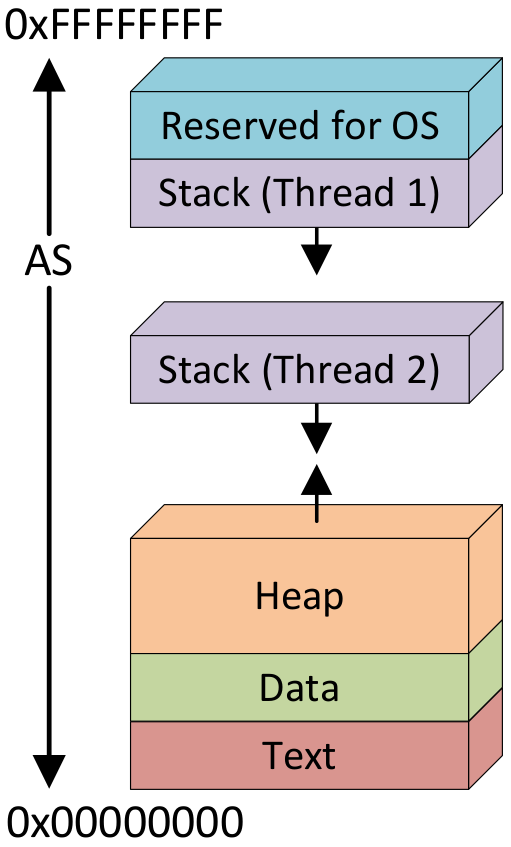
\includegraphics[width=0.15\textwidth]{KLTAddressSpace}\end{figure}

\paragraph{Thread models --- M:N}
\begin{itemize}
  \item \textbf{Principle}: \( M \) ULTs are maps to (at most) \( N \) KLT
  \begin{itemize}
    \item \emph{Goal}: pros of ULT and KLT --- non-blocking with quick management
    \item create sufficient number of KLTs and flexibly allocate ULTs to them
    \item \emph{Idea}: if ULT blocks ULTs can be switched in userspace
  \end{itemize}
  \item \textbf{Pros}:
  \begin{itemize}
    \item[+] flexible scheduling policy
    \item[+] efficient execution
  \end{itemize}
  \item \textbf{Cons}:
  \begin{itemize}
    \item[-] hard to debug
    \item[-] hard to implement (e.g. blocking, number of KLTs,\dots)
  \end{itemize}
  \item \textbf{Implementation --- Up-calls}:
  \begin{itemize}
    \item kernel notices that thread will block \( \to \) sends signal to process
    \item up-call notifies process of thread id and event that happened
    \item exception handler of process schedules a different process thread
    \item kernel later informs process that blocking event finished via other up-call
  \end{itemize}
\end{itemize}

\begin{summary}
  \begin{itemize}
    \item programs often do closely related things at once
    \begin{itemize}
      \item mapped to thread abstraction: multiple threads of execution operate in same process
    \end{itemize}
    \item differentiation between process information (PCB) and thread information (TCB)
    \item \textbf{thread models}:
    \begin{itemize}
      \item $ N:1 $: threads fully managed in user-space
      \item $ 1:1 $: threads fully managed by kernel
      \item $ M:N $: threads are flexibly managed either in user-space or kernel
    \end{itemize}
    \item multi-threaded programs operate on same data concurrently or even parallel:
    \begin{itemize}
      \item \emph{synchronization}: accessing such data must be synchronized
      \item[$ \to $] makes writing such programs challenging
    \end{itemize}
  \end{itemize}
\end{summary}


  % \section{Scheduling}

\paragraph{Motivation}
\begin{items}
  \item \( K \) jobs ready to run, \( K > N \geq 1 \) CPUs available
  \item \textbf{Scheduling Problem}: \\*
    - Which jobs should kernel assign to which CPUs? \\*
    - When should it make decision?
\end{items}

\paragraph{Dispatcher}
\begin{items}
  \item \textbf{Dispatcher}: performs actual process switch \\*
    - mechanism \\*
    - save/restore process context \\*
    - switch to user mode
  \item \textbf{Scheduler}: selects next process to run based on \emph{policy}
\end{items}

\paragraph{Voluntary Yielding vs. Preemption}
\begin{items}
  \item kernel responsible for CPU switch
  \item kernel doesn't always run \( \to \) can only dispatch different process when invoked
  \item \textbf{cooperative multitasking}: running process performs \emph{yield} syscall \( \to \) kernel switches process
  \item \textbf{preemptive scheduling}: \\*
    - kernel invoked in certain time intervals \\*
    - kernel makes scheduling decisions after every time-slice
\end{items}
\begin{figure}[H]\centering\label{ProcessSwitching}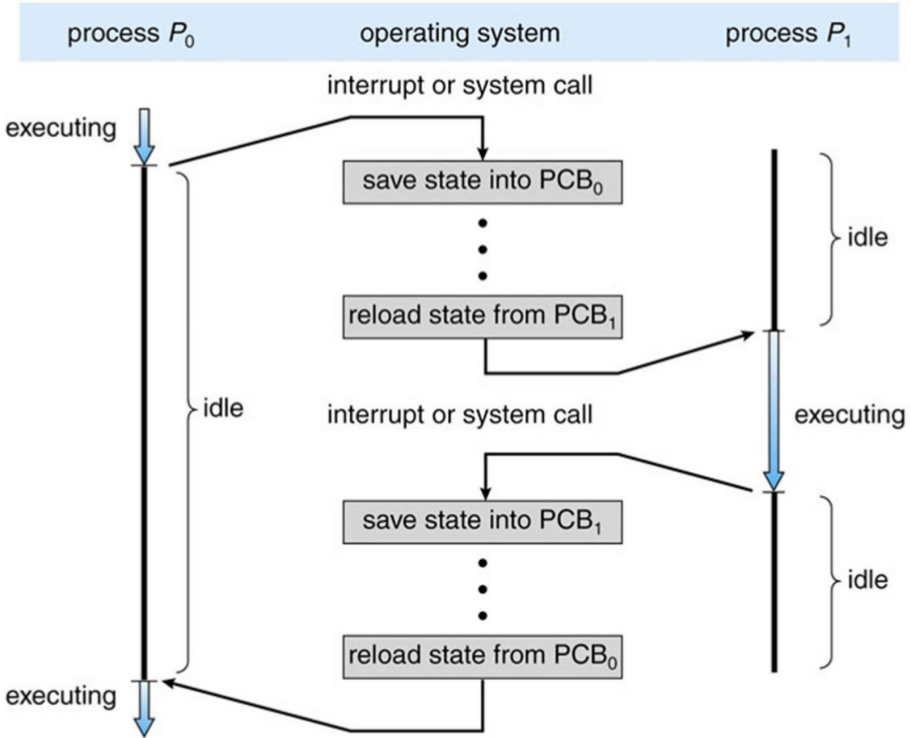
\includegraphics[width=0.33\textwidth]{ProcessSwitching}\end{figure}

\paragraph{Scheduling --- Process States}
\begin{items}
  \item \textbf{new}: process was created but did not run yet
  \item \textbf{running}: instructions are currently being executed
  \item \textbf{waiting}: process is waiting for some event
  \item \textbf{ready}: process is waiting to by assigned a processor
  \item \textbf{terminated}: process has finished execution
\end{items}

\paragraph{Scheduling --- long-term vs. short-term}
\begin{items}
  \item \textbf{Short-term scheduler} (CPU Scheduler, focused on in this lecture): \\*
    - selects process to run next, allocates CPU \\*
    - invoked frequently (ms) \( \leadsto \) must be fast
  \item \textbf{Long-term scheduler} (job scheduler): \\*
    - selects process to be brought into ready queue \\*
    - invoked very infrequently (s, m) \( \leadsto \) can be slow \\*
    - controls degree of \emph{multiprogramming}
\end{items}

\paragraph{Scheduling queues}
\begin{items}
  \item \textbf{job queue}: set of all processes in system
  \item \textbf{ready queue}: process in main memory, ready or waiting
  \item \textbf{device queue}: processes waiting for I/O device
\end{items}

\paragraph{Scheduling Policies --- Categories}
\begin{items}
  \item \textbf{batch scheduling}: \\*
    - still widespread in business (payroll, inventory,\dots) \\*
    - no users waiting for quick response \\*
    - non-preemptive algorithms acceptable \( \to \) less switches \( \to \) less overhead
  \item \textbf{interactive scheduling}: \\*
    - need to optimize for response time \\*
    - preemption essential to keep processes from hogging CPU
  \item \textbf{real-time scheduling}: \\*
    - guarantee job completion within time constraints \\*
    - need to be able to plan when which process runs + how long \\*
    - preemption not always needed
\end{items}

\paragraph{Scheduling Policies --- Goals}
\begin{items}
  \item \textbf{General}: \\*
    - \emph{fairness}: give each process fair share of CPU \\*
    - \emph{balance}: keep all parts of system busy
  \item \textbf{batch scheduling}: \\*
    - \emph{throughput}: number of processes that complete per time unit \\*
    - \emph{turnaround time}: time from job submission to job completion \\*
    - \emph{CPU utilization}: keep CPU as busy as possible
  \item \textbf{interactive scheduling}: \\*
    - \emph{waiting time}: reduce time a process waits in waiting queue \\*
    - \emph{response time}: time from request to first response
  \item \textbf{real-time scheduling}: \\*
    - \emph{meeting deadlines}: finishing jobs in time \\*
    - \emph{predictability}: minimize jitter
\end{items}

\paragraph{Scheduling Policies --- first come first served}
\begin{items}
  \item intuitively clear
  \item \textbf{Example}: 3 processes arrive at time 0 in the order \( P_1, P_2, P_3 \)
    \begin{center}
      \begin{tabular}{|c|c|c|}
        \textbf{Process} & \textbf{Burst time} & \textbf{Turnaround time} \\
        \hline
        \( P_1 \) & 24 & 24 \\
        \( P_2 \) & 3 & 27 \\
        \( P_3 \) & 3 & 30
      \end{tabular}
    \end{center}
  \item \( \leadsto \) average turnaround time 27 \( \to \) \emph{can we do better?}
  \item \textbf{Conclusion}: if processes would arrive in order \( P_2 \), \( P_3 \), \( P_1 \), average turnaround time would be 13 \\*
    \( \leadsto \) \emph{good scheduling can reduce turnaround time}
\end{items}

\paragraph{Scheduling Policies --- shortest job first}
\begin{items}
  \item \textbf{Benefits}: optimal average turnaround/waiting/response time
  \item \textbf{Challenge}: cannot know job lengths in advance
  \item \textbf{Solution}: predict length of next CPU burst for each process \\*
    \( \leadsto \) schedule process with shortest burst next
  \item \textbf{Burst Estimation}: \emph{exponential averaging} \\*
    - \( \tau_{n+1} = \alpha t_n + (1-\alpha)\tau_n \) \\* \phantom{-} (\( t_n \): actual length of \( n \)-th CPU burst, \( \tau_{n+1} \): predicted length of next CPU burst, \( 0 \leq \alpha \leq 1 \))
\end{items}

\paragraph{Process Behavior --- CPU bursts}
\begin{items}
  \item CPU bursts exists because processes wait for I/O
  \item \textbf{CPU-bound processes}: spends more time doing computations \\*
    \( \leadsto \) few very long CPU bursts
  \item \textbf{I/O-bound processes}: spends more time doing I/O \\*
    \( \leadsto \) many short CPU bursts
\end{items}

\paragraph{Scheduling Policies --- preemptive shortest-job-first}
\begin{items}
  \item SJF optimizes waiting/response time \\*
    \( \leadsto \) what about throughput?
  \item \textbf{Problem}: CPU-bound jobs hold CPU until exit or I/O \( \to \) \emph{poor I/O utilization}
  \item \textbf{Idea}: SJF, but preempt periodically to make new scheduling decision \\*
    - each time slice: schedule job with shortest remaining time next \\*
    - alternatively: schedule job with shortest next CPU burst
\end{items}

\paragraph{Scheduling Policies --- round robin}
\begin{items}
  \item \textbf{Problem}: batch schedulers suffer from starvation and don't provide fairness
  \item \textbf{Idea}: each process runs for small CPU time unit \\*
    - \emph{time quantum}/\emph{time slice} length: usually 10-100ms \\*
    - preempt processes that have not blocked by end of time slice \\*
    - append current thread to end of run queue, run next thread
  \item \textbf{Caution}: time slice length needs to balance interactivity and overhead! \\*
    \( \to \) if time slice length in the area of dispatch time, 50\% of CPU time wasted for process switching
\end{items}

\paragraph{Scheduling Policies --- virtual round robin}
\begin{items}
  \item \textbf{Problem}: RR is unfair for I/O-bound jobs: they block before using up time quantum
  \item \textbf{Idea}: put jobs that didn't use up their quantum in additional queue \\*
    - store share of unused time-slice \\*
    - give those jobs additional queue priority \\*
    - put them back into normal queue afterwards
\end{items}

\paragraph{Scheduling Policies --- (strict) priority scheduling}
\begin{items}
  \item \textbf{Problem}: not all jobs are equally important \\*
    \( \leadsto \) different priorities (e.g., 4)
  \item \textbf{Solution}: associate priority number with each process \\*
    - RR for each priority \\*
    - \emph{aging}: old low priority processes get executed before new higher priority processes
\end{items}

\paragraph{Scheduling Policies --- multi-level feedback queue}
\begin{items}
  \item \textbf{Problem}: context switching expensive \\*
    \( \leadsto \) trade-off between interactivity and overhead?
  \item \textbf{Goals}: \\*
    - higher priority for I/O jobs (usually don't use up quantum) \\*
    - low priority for CPU jobs (rather run them longer)
  \item \textbf{Idea}: different queues with different priorities and time slice lengths \\*
    - schedule queues with (static) priority scheduling \\*
    - double time slice length in each next-lower priority \\*
    - process to higher priority when they don't use up quantum repetitively \\*
    - process to lower priority when they use up quantum repetitively
\end{items}

\paragraph{Scheduling Principles --- priority donation}
\begin{items}
  \item \textbf{Problem}: Process B (higher priority) waits for process A (lower priority) \\*
    \( \leadsto \) B has now effectively lower priority
  \item \textbf{Solution}: \emph{priority donation} \\*
    - give A priority of B as long as B waits for A \\*
    - if C, D, E wait for B \( \to \) A gets highest priority of B, C, D, E
\end{items}

\paragraph{Scheduling Policies --- lottery scheduling}
\begin{items}
  \item issue number of lottery tickets to processes (amount depending on priority)
  \item amount of tickets controls average proportion of CPU for each process
  \item \textbf{Scheduling}: scheduler draws random number \( N \), process with \( N \)-th ticket is executed
  \item processes can transfer tickets to other processes if they wait for them
\end{items}

\begin{summary}
  \begin{items}
    \item \textbf{phases}: processes have phases of communication and waiting for I/O \\*
      $ \to $ appropriate switching between processes increases computing system utilization
    \item \textbf{goal-based}: scheduler decides what appropriate means based on goals \\*
      $ - $ \emph{long-term scheduler}: degree of multiprogramming \\*
      $ - $ \emph{short-term scheduler}: which process to run next
    \item \textbf{dispatching}: only happens when OS is invoked \\*
      $ - $ \emph{cooperative scheduling}: currently running thread yields (syscall) \\*
      $ - $ \emph{preemptive scheduling}: OS is called periodically to switch threads
  \end{items}
\end{summary}

  % \section{Inter Process Communication}

\paragraph{Overview}
\begin{items}
  \item \textbf{Reassons} for cooperating processes: \\*
    - \emph{information sharing}: share file/data-structure in memory \\*
    - \emph{computation speed-up}: break large tasks in subtasks \( \leadsto \) parallel execution \\*
    - \emph{modularity}: divide system into collborating modules with clean interfaces
  \item \textbf{IPC}: allows data exchange \\*
    - \emph{message passing}: explicity send/receive information using syscalls \\*
    - \emph{shared memory}: physical memory region used by multiple processes/threads
\end{items}

\paragraph{IPC --- message passing}
\begin{items}
  \item = mechanism for processes to communicate and synchronize
  \item message passing facilities generally provide \code{send} and \code{receive}
  \item \textbf{Implementations}: \\*
    - hardware bus \\*
    - shared memory \\*
    - kernel memory \\*
    - network interface card (NIC)
  \item \textbf{Direct messages}: processes explicitly named when exchanging messages
  \item \textbf{Indirect messages}: sending to/receiving from \emph{mailboxes} \\*
    - first communicating process creates mailbox, last destroys \\*
    - processes can only communicate through shared mailbox
\end{items}

\paragraph{Indirect messages -- synchronization}
\begin{items}
  \item \textbf{Blocking} (synchronous): \\*
    - \emph{blocking send}: sender blocks until message is received \\*
    - \emph{blocking receive}: receiver blocks until message is available
  \item \textbf{Non-blocking} (asynchronous): \\*
    - \emph{non-blocking send}: sender sends message, then continues \\*
    - \emph{non-blocking receive}: receiver receives valid message or \code{null}
\end{items}

\paragraph{Messaging --- Buffering}
\begin{items}
  \item messages are \emph{queued} using different capacities while being in-flight
  \item \textbf{zero capacity}: no queuíng \\*
    - \emph{rendezvous}: sender must wait for receiver \\*
    - message is transferred as soon as receiver becomes available \( \to \) no latency/jitter
  \item \textbf{bounded capacity}: finite number + length of messages \\*
    - sender can send before receiver waits for messages \\*
    - sender must wait if link is full
  \item \textbf{unbounded capacity}: \\*
    - sender never waits \\*
    - memory may overflow \( \to \) potentially large latency/jitter between \code{send} and \code{receive}
\end{items}

\paragraph{Messaging --- POSIX message queues}
\begin{items}
  \item \textbf{create} or open existing message queue: \\*
    \code{mqd_t mq_open (const char *name, int oflag);} \\*
    - \code{name} ist path in file system \\*
    - access permission controlled through file system access permission
  \item \textbf{send} message to message queue: \\*
    \code{int mq_send (mqd_t md, const char *msg, size_t len, unsigned priority);}
  \item \textbf{receive} message with highest priority in message queue: \\*
    \code{int mq_receive (mqd_t md, char *msg, size_t len, unsigned *priority);}
  \item \textbf{register} callback handler on message queue (to avoid polling): \\*
    \code{int mq_notify (mqd_t md, const struct sigevent *sevp);}
  \item \textbf{remove} message queue: \\*
    \code{int mq_unlink (const char *name);}
\end{items}

\paragraph{Shared Memory}
\begin{items}
  \item \textbf{Principle}: communicate through region of shared memory \\*
    - every write to shared region is visible to all other processes \\*
    - hardware guarantees that always most recent write is read
  \item \textbf{Implementation}: message passing via shared memory is application-specific
  \item \textbf{Problems}: using shared memory in a safe way is tricky \\*
    - \emph{cache coherency protocol}: makes usage with many processes/CPUs hard \\*
    - \emph{race conditions}: makes usage with multiple writers hard
\end{items}

\paragraph{Shared Memory --- POSIX shared memory}
\begin{items}
  \item \textbf{create} or open existing POSIX shared memory object: \\*
    \code{int shm_open (const char *name, int oflag, mod_t mode);}
  \item \textbf{set} size of shared memory region: \\*
    \code{ftruncate (smd, size_t len);}
  \item \textbf{map} shared memory object to address space: \\*
    \code{void* mmap (void* addr, size_t len, [...], smd, [...]);}
  \item \textbf{unmap} shared memory object from address space: \\*
    \code{int munmap (void* addr, size_t len);}
  \item \textbf{destroy} shared memory object: \\*
    \code{int shm_unlink (const char *name);}
\end{items}

\paragraph{Shared Memory --- sequential memory consistency}
\begin{items}
  \item = \emph{the result of execution as if all operations were executed in some sequential order, and the operations of each processor occurred in the order specified by the program.}
  \item \textbf{Model}: \\*
    - all memory operations occur one at a time in \emph{program order} \\*
    - ensures write atomicity
  \item \textbf{Reality}: compiler and CPU re-order instructions to \emph{execution order} \\*
    \( \to \) without SC many processes on many CPU behave worse than preemptive threads on 1 CPU
\end{items}

\paragraph{Shared Memory --- memory consistency model}
\begin{items}
  \item \textbf{Problem}: \\*
    - CPUs generally not sequentially consistent \\*
    - compilers do not generate code in program order
\end{items}

\paragraph{Syncronization --- race conditions}
\begin{items}
  \item \textbf{Assume}: sequential memory consistency \( \to \) no atomic memory transactions!
  \item \textbf{Critical Sections}: protect instructions inside critical section from concurrent execution
\end{items}

\paragraph{Critical Sections --- desired properties}
\begin{items}
  \item \textbf{mutual exclusion}: at most one thread can be in the CS at any time
  \item \textbf{progress}: no thread running outside of CS may block another thread from getting in
  \item \textbf{bounded waiting}: once a thread starts trying to enter CS, there is a bound on number of times other threads get in
\end{items}

\paragraph{Critical Sections --- disabling interrupts}
\begin{items}
  \item kernel only switches on interrupts (usually on \emph{timer interrupt}) \\*
    \( \to \) have per-thread \emph{do not interrupt} (DNI)-bit
  \item \textbf{single-core system}: \\*
    - enter CS: set DNI bit \\*
    - leave CS: clear DNI bit
  \item \textbf{Advantages}: \\*
    - easy + convenient in kernel
  \item \textbf{Disadvantages}: \\*
    - \emph{only works on signle-core systems}: disabling interrupts on one CPU doesn't affect other CPUs \\*
    - \emph{only feasible in kernel}: don't want to give user power to turn off interrupts!
\end{items}

\paragraph{Critical Sections --- lock variables}
\begin{items}
  \item define global \code{lock} variable \\*
    - only enter CS if \code{lock} is \code{0}, set to \code{1} on enter \\*
    - wait for lock to become \code{0} otherwise (\emph{busy waiting})
  \item \textbf{Problem}: doesn't solve CS problem! Reading/Setting lock not atomic!
\end{items}

\paragraph{Critical Sections --- spinlocks}
\begin{items}
  \item to make lock variable approach work, lock variable must be tested and set at same time atomically:
  \item \textbf{x86}: \code{xchg} can atomically exchange memory content with register \\*
    - exchanges register content with memory content \\*
    - returns previous memory content of lock \\*
    \( \leadsto \) implementation of critical section as \emph{spinlock}:
  \begin{lstlisting}[language=c]
void enter_critical_section (volatile bool *lock) {
  while (xchg(lock, 1) == 1); // lock = 1 and return old value
                                 // repeat until old value != 1
}

void leave_critical_section (volatile bool *lock) {
  *lock = 0;
}
  \end{lstlisting}
  \item \textbf{Advantages}: \\*
    - \emph{mutual exclusion}: only one thread can enter CS \\*
    - \emph{progress}: only thread within CS hinders others of getting in
  \item \textbf{Disadvantages}: \\*
    - \emph{bounded waiting}: no upper bound
\end{items}

\paragraph{Spinlocks --- Limitations}
\begin{items}
  \item \textbf{Congestion}: \\*
    - if most times there is no thread in CS when another tries to enter, then spinlocks are \\* \phantom{-} \phantom{\( \cdot \)} very easy + efficient \\*
    - if CS is large or many threads try to enter, spinlocks might not be good choice as all \\* \phantom{-} \phantom{\( \cdot \)} threads actively wait spinning
  \item \textbf{Multicore}: memory address is written at every atomic swap operation \\*
    \( \to \) memory is expensively kept coherent 
  \item \textbf{Static Priorities} (e.g., \emph{priority inversion}): if low-priority threads hold lock it will never be able to release it, because it will never be scheduled
\end{items}

\paragraph{Spinlocks --- sleep while wait}
\begin{items}
  \item \textbf{Problem}: busy part of busy waiting \\*
    - wastes resources, \\*
    - stresses cache coherence protocol, \\*
    - can cause priority inversion problem
  \item \textbf{Idea}: \\*
    - threads sleep on locks if occupied \\*
    - wake up threads one at a time when lock becomes free
\end{items}

\paragraph{Spinlocks --- semaphore}
\begin{items}
  \item two new syscalls operating on \code{int} variables: \\*
    - \code{wait (&s)}: if \code{s > 0}: \code{s--} and continue, otherwise let caller sleep \\*
    - \code{singal (&s)}: if no thread is waiting: \code{s++}, otherwise wake one up
  \item initialize \code{s} to maximum number of threads that may enter CS \\*
    - \code{wait} = \code{enter_critical_section()} \\*
    - \code{signal} = \code{leave_critical_section()}
  \item \textbf{mutex} (semaphore): semaphore initialized to 1 (only admits one thread at a time into CS)
  \item \textbf{counting semaphore}: semaphore allowing more than one thread into CS at a time
\end{items}

\paragraph{Semaphore --- implementation}
\begin{items}
  \item \code{wait} and \code{signal} calls need to be carefully synchronized (otherwise \emph{race condition} between checking and decrementing \code{s})
  \item \textbf{signal loss} can occur when waiting and waking threads up at same time
  \item \( \leadsto \) each semaphore has \textbf{wake-up queue}: \\*
    - \emph{weak semaphores}: wake up random waiting thread on \code{signal} \\*
    - \emph{strong semaphores}: wake up thread strictly in order which they started \code{wait}ing
  \item \textbf{Advantages}: \\*
    - \emph{mutual exclusion}: only one thread can enter CS for mutexes \\*
    - \emph{progress}: only thread within CS hinders others to get in \\*
    - \emph{bounded waiting}: strong semaphores guarantee bounded waiting
  \item \textbf{Disadvantages}: \\*
    - every enter and exit of CS is syscall \( \to \) slow
\end{items}

\paragraph{Fast User Space mutex}
\begin{items}
  \item \textbf{spinlock}: \\*
    + quick when wait-time is short \\*
    - waste resources when wait-time is long
  \item \textbf{semaphore}: \\*
    + efficient when wait-time is long \\*
    - syscall overhead at every operation
  \item \textbf{futex}: \\*
    - userspace + kernel component \\*
    - try to get into CS with userspace spinlock \\*
    \phantom{-} \( \cdot \) CS busy \( \to \) use syscall to put thread to sleep \\*
    \phantom{-} \( \cdot \) otherwise \( \to \) enter CS with now locked spinlock completely in userspace
\end{items}

  % \section{Synchronization and Deadlocks}

\paragraph{Producer-Consumer Problem}
\begin{items}
  \item \textbf{Definition}: \\*
    $ - $ buffer is shared between producer and consumer (LIFO) \\*
    $ - $ \code{count} integer keeps track of number of currently available items \\*
    $ - $ producer produces item $ \to $ placed in buffer, \code{count++} \\*
    $ - $ buffer full $ \to $ producer needs to sleep until consumer consumed an item \\*
    $ - $ consumer consumes item $ \to $ remove item from buffer, \code{count--} \\*
    $ - $ buffer empty $ \to $ consumer needs to sleep until producer produces item
  \item \textbf{Problem}: \emph{race condition} on \code{count}
\end{items}

\paragraph{Producer-Consumer Problem --- condition variables}
\begin{items}
  \item \textbf{Solution}: can be solved with mutex + 2 counting semaphores \\*
    $ - $ hard to understand \\*
    $ - $ hard to get right \\*
    $ - $ hard to transfer to other problems
  \item \textbf{condition variables}: allow blocking until condition is met \\*
   $ - $ usually suitable for same problems but much easier to get right
  \item \textbf{Idea}: \\*
    $ - $ new operation performs \emph{unlock}, \emph{sleep}, \emph{lock} atomically \\*
    $ - $ new wake-up operation is called with lock held \\*
    $ \to $ simple mutex lock/unlock around CS + no signal loss
  \item \textbf{Pthread} condition variables: \\*
    $ - $ \code{pthread_cond_init}: create + initialize new CV \\*
    $ - $ \code{pthread_cond_destroy}: destroy + free existing CV \\*
    $ - $ \code{pthread_cond_wait}: block waiting for signal \\*
    $ - $ \code{pthread_cond_timedwait}: block waiting for signal or timer \\*
    $ - $ \code{pthread_cond_signal} : signal another thread to wake up \\*
    $ - $ \code{pthread_cond_broadcast}: signal all threads to wake up
\end{items}
\begin{figure}[H]\centering\label{ConditionVariables}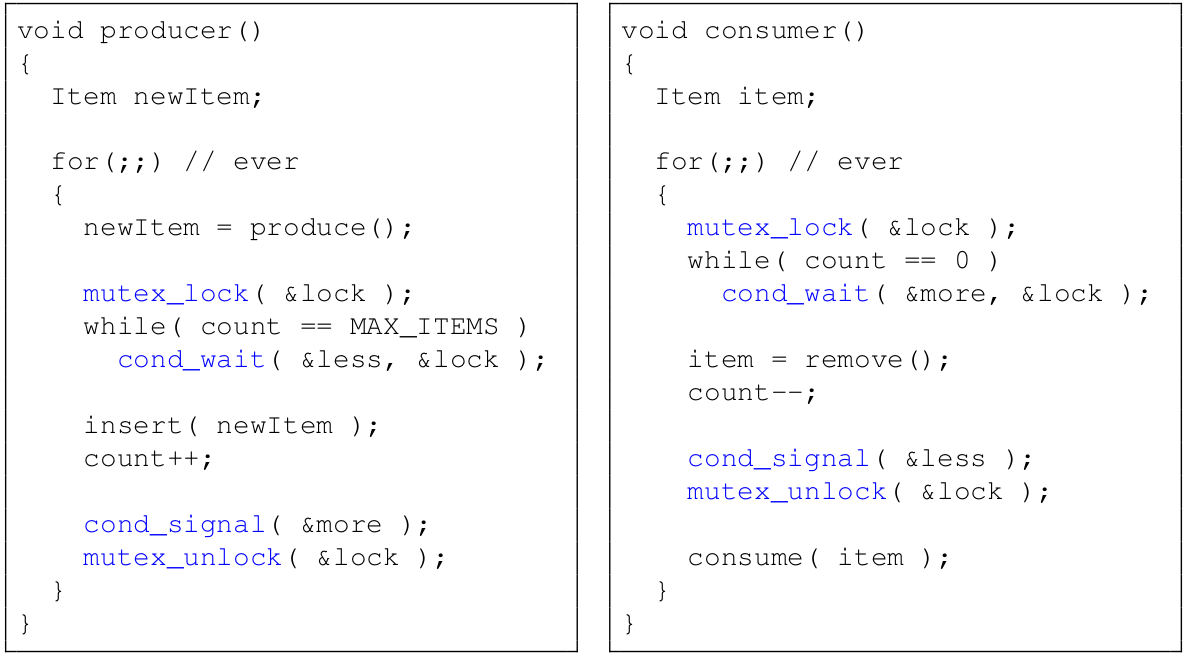
\includegraphics[width=0.33\textwidth]{ConditionVariables}\end{figure}

\paragraph{Reader-Writer Problem}
\begin{items}
  \item \textbf{Problem}: model access to shared data structures \\*
    $ - $ many threads compete to read/write same data \\*
    $ - $ \emph{readers}: only read data set, not performing any updates \\*
    $ - $ \emph{writers}: both read and write \\*
    $ \leadsto $ using single mutex for read/write operations is not a good solution! \\*
    \phantom{$ \leadsto $} (unnecessarily blocking out multiple readers while no writer is present)
  \item \textbf{Idea}: locking should reflect different semantics for reading/writing \\*
  $ - $ no writing thread $ \to $ multiple readers may be present \\*
  $ - $ writing thread $ \to $ no other reader/writer allowed
\end{items}

\paragraph{Dining-Philosophers Problem}
\begin{items}
  \item \textbf{Definition}: 5 philosophers with cyclic workflow: \\*
    $ - $ think \\*
    $ - $ get hungry \\*
    $ - $ grab one chopstick \\*
    $ - $ grab other chopstick \\*
    $ - $ eat \\*
    $ - $ put down chopsticks
  \item \textbf{Rules}: \\*
    $ - $ no communication \\*
    $ - $ no atomic grabbing of both chopsticks \\*
    $ - $ no wrestling
  \item \textbf{Abstraction}: models threads competing for limited number of resources
  \textbf{Problem}: what happens if all philosophers grab left chopstick at once?
  \item \textbf{Deadlock workarounds}:  \\*
    $ - $ just 4 philosophers allowed at table of 5 $ \to $ \emph{deadlock avoidance} \\*
    $ - $ odd philosophers take left chopstick first, even ones take right first $ \to $ \emph{deadlock prevention}
\end{items}
\begin{figure}[H]\centering\label{DiningPhilosophers}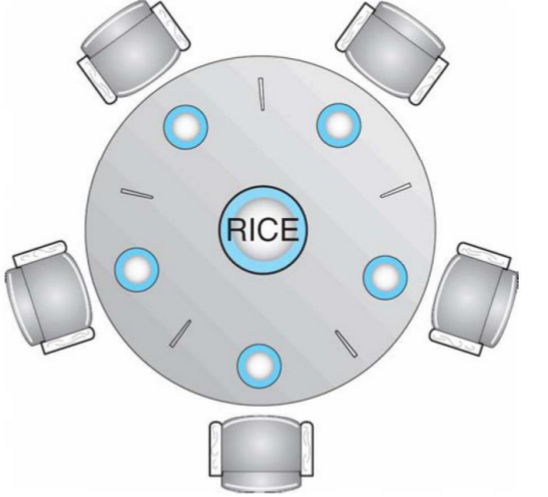
\includegraphics[width=0.2\textwidth]{DiningPhilosophers}\end{figure}

\paragraph{Deadlocks}
\begin{items}
  \item \textbf{Deadlocks} can arise if all four conditions hold simultaneously: \\*
    $ - $ \emph{mutual exclusion}: limited resource access (can only be shared with finite number of users) \\*
    $ - $ \emph{hold and wait}: wait for next resource while already holding at least one \\*
    $ - $ \emph{no preemption}: granted resource cannot be taken away but only handled back voluntarily \\*
    $ - $ \emph{circular wait}: possibility of circularity in requests graph
\end{items}

\paragraph{Deadlocks --- countermeasures}
\begin{items}
  \item \textbf{prevention}: pro-active, make deadlocks impossible to occur
  \item \textbf{avoidance}: decide on allowed actions based on a-priori knowledge
  \item \textbf{detection} (\emph{recovery}): react after deadlock happened
\end{items}

\paragraph{Deadlocks --- prevention}
\begin{items}
  \item \textbf{Goal}: negate at least one of the required deadlock conditions: \\*
    $ - $ \emph{mutual exclusion}: buy more resources, split into pieces, virtualize \\*
    $ - $ \emph{hold and wait}: get all resources en-bloque, 2-phase-locking \\*
    $ - $ \emph{no preemption}: virtualize to make preemptable \\*
    $ - $ \emph{circular wait}: reorder resources, prevent through partial order on resources
\end{items}

\paragraph{Deadlocks --- avoidance}
\begin{items}
  \item \textbf{safe state}: system is in safe state $ \to $ no deadlocks
  \item \textbf{unsafe state}: system is in unsafe state $ \to $ deadlocks possible
  \item \textbf{avoidance}: on every resource request decide if system stays in safe state \\*
    $ \to $ \emph{resource allocation graph}
\end{items}

\paragraph{Deadlock Avoidance --- resource allocation graph}
\begin{items}
  \item \textbf{principle}: view system state as graph \\*
    $ - $ \emph{processes} = round nodes \\*
    $ - $ \emph{resources} = square nodes \\*
    $ - $ \emph{resource instance} = dot in resource node \\*
    $ - $ \emph{resource requests/assignments} = edges \\*
    \phantom{$ - $} $ \cdot $ resource $ \to $ process = resource is assigned to process \\*
    \phantom{$ - $} $ \cdot $ process $ \to $ resource = process is requesting resource
  \begin{figure}[H]\centering\label{ResourceAllocationGraph}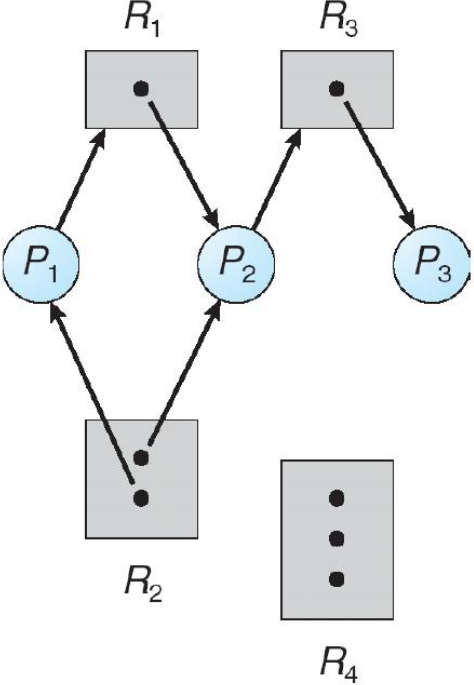
\includegraphics[width=0.15\textwidth]{ResourceAllocationGraph}\end{figure}
\end{items}

\paragraph{Deadlocks --- detection}
\begin{items}
  \item \textbf{principle}: allow system to enter deadlock $ \to $ detection $ \to $ recovery scheme
  \item \textbf{wait-for graph} (WFG): \\*
    $ - $ \emph{processes} = nodes \\*
    $ - $ \emph{wait-for relationship} = edges
  \item periodically invoke algorithm searching for cycle in graph \\*
    $ \leadsto $ cycle exists $ \to $ deadlock exists
\end{items}
\begin{figure}[H]\centering\label{WaitForGraph}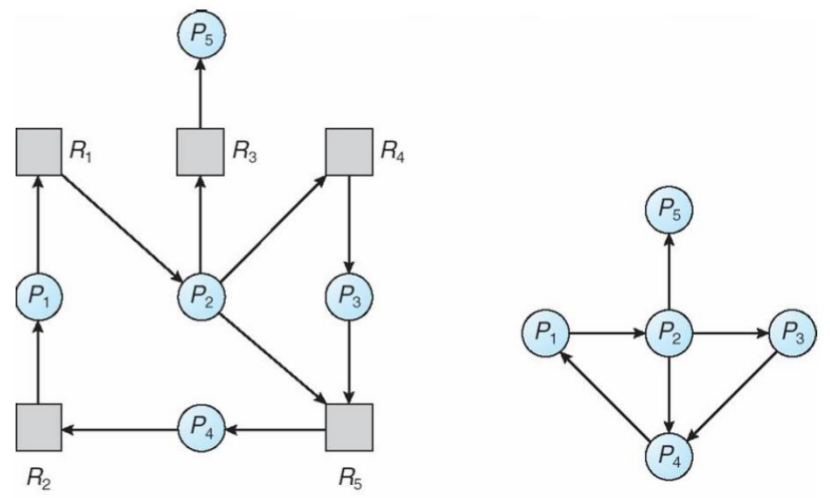
\includegraphics[width=0.33\textwidth]{WaitForGraph}\end{figure}

\paragraph{Deadlocks --- recovery}
\begin{items}
  \item \textbf{process termination}: \\*
    $ - $ \emph{all}: abort all deadlocked processes \\*
    $ - $ \emph{selective}: abort one process at a time until deadlock is eliminated
  \item \textbf{termination order}: in which order should processes be aborted? \\*
    $ - $ process priority \\*
    $ - $ how long already computed? how much longer for completion? \\*
    $ - $ amount of resources used \\*
    $ - $ amount of resources needed for completion \\*
    $ - $ how many processes will need to be terminated \\*
    $ - $ interactive or batch?
  \item \textbf{resource preemption}: \\*
    $ - $ \emph{victim selection}: minimize cost \\*
    $ - $ \emph{rollback}: perform periodic snapshots, abort process to preempt resources $ \to $ restart from last \\* \phantom{$ - $} \phantom{$ \cdot $} safe state \\*
    $ - $ \emph{starvation}: same process may always be picked as victim $ \leadsto $ include rollback count in cost factor
\end{items}

\begin{summary}
  \begin{items}
    \item \textbf{classical synchronization problems}: model synchronization problems occurring in reality \\*
      $ - $ \emph{producer-consumer}: shared use of buffers/queues \\*
      $ - $ \emph{reader-writer}: shared access to data structures \\*
      $ - $ \emph{dining philosophers}: competition for limited resources
    \item such synchronization problems occur very often when programming operating systems
    \item \textbf{parallelism}: introduced by multiple processors + multiprogramming, needs to be considered carefully when writing OS
  \end{items}
\end{summary}

  % \section{Memory Management Hardware}

\paragraph{Main Memory}
\begin{itemize}
  \item main memory + registers = only storage that CPU can access directly
  \item \textbf{Before run}: program must be
  \begin{itemize}
    \item brought into memory from background storage
    \item placed within a process' address space
  \end{itemize}
  \item \textbf{Earlier}: computers had no memory abstraction
  \begin{itemize}
    \item[$ \to $] programs accessed physical memory directly
  \end{itemize}
  \item multiple processes can be run concurrently even without memory abstraction (using swapping, relocation)
\end{itemize}

\paragraph{Swapping}
\begin{itemize}
  \item \textbf{Principle}:
  \begin{itemize}
    \item \emph{roll-out}: save program's state on background storage
    \item \emph{roll-in}: replace program state with another program's state
  \end{itemize}
  \item \textbf{Advantages}:
  \begin{itemize}
    \item[+] only needs hardware support to protect kernel, not to protect processes from one another
  \end{itemize}
  \item \textbf{Disadvantages}:
  \begin{itemize}
    \item[-] \emph{very slow}: major part of swap time is transfer time
    \item[-] \emph{no parallelism}: only one process runs at a time, owns entire physical address space
  \end{itemize}
\end{itemize}

\paragraph{Overlays}
\begin{itemize}
  \item \textbf{Problem}: what if process needs more memory than available?
  \begin{itemize}
    \item[$ \to $] need to partition program manually
  \end{itemize}
\end{itemize}

\paragraph{Static Relocation}
\begin{itemize}
  \item[=] OS adds fixed offset to every address in a program when loading + creating process
  \item same address space for every process
  \begin{itemize}
    \item[$ \to $] \emph{no protection}: every program sees + can access every address!
  \end{itemize}
\end{itemize}

\paragraph{Shared Physical Memory --- Goals}
\begin{itemize}
  \item \textbf{Protection}:
  \begin{itemize}
    \item bug in one process must not corrupt memory in another
    \item do not allow processes to observe other processes' memory
  \end{itemize}
  \item \textbf{Transparency}:
  \begin{itemize}
    \item process should not require particular physical memory addresses
    \item processes should not be able to use large amounts of contiguous memory
  \end{itemize}
  \item \textbf{Resource Exhaustion}: allow that sum of sizes of all processes is greater than physical memory
\end{itemize}

\paragraph{Memory Management Unit}
\begin{itemize}
  \item \textbf{Motivation}: need hardware support to achieve safe + secure protection
  \item \textbf{Goal}: hardware maps virtual to physical address
  \item \textbf{Usage}: user program deals with virtual addresses, never sees real addresses
\end{itemize}
\begin{figure}[h]\centering\label{MMU}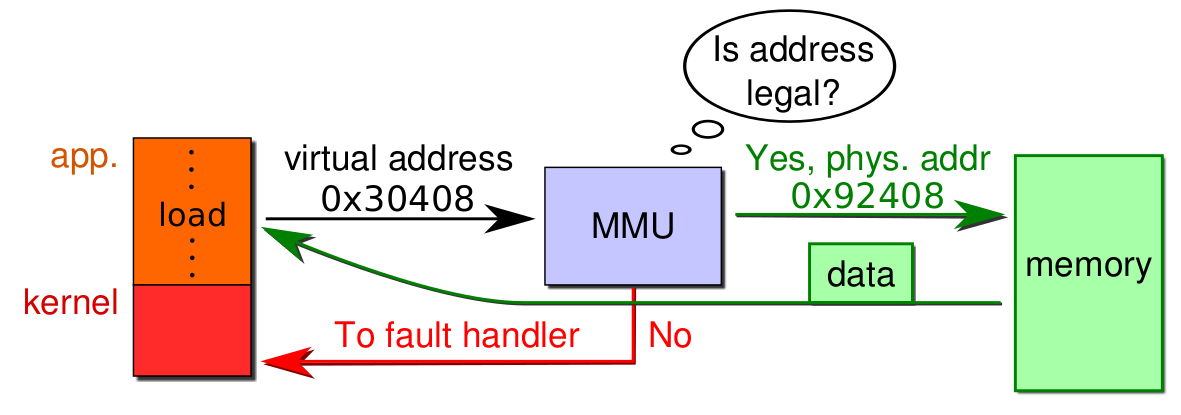
\includegraphics[width=0.33\textwidth]{MMU}\end{figure}

\paragraph{MMU --- base and limit registers}
\begin{itemize}
  \item \textbf{Idea}: provide protection + dynamic relocation in MMU
  \begin{itemize}
    \item[$ \to $] introduce special \emph{base} and \emph{limit} registers (e.g., Cray-1)
  \end{itemize}
  \item \textbf{Usage}: on every load/store the MMU 
  \begin{itemize}
    \item checks if virtual address \( \geq \) \code{base}
    \item checks if virtual address \( < \) \code{base} + \code{limit}
    \item use virtual address as physical address in memory
  \end{itemize}
  \item \textbf{Protection}: OS needs to be protected from processes
  \begin{itemize}
    \item main memory split in two partitions (low = OS, high = user processes)
    \item OS can access all process partitions (e.g., to copy syscall parameters)
    \item MMU denies processes access to OS memory
  \end{itemize}
  \item \textbf{Advantages}:
  \begin{itemize}
    \item[+] straight forward to implement MMU
    \item[+] very quick at run-time
  \end{itemize}
  \item \textbf{Disadvantages}:
  \begin{itemize}
    \item[+] how to grow process' address space?
    \item[+] how to share code/data?
  \end{itemize}
\end{itemize}
\begin{figure}[h]\centering\label{MMUBaseLimit}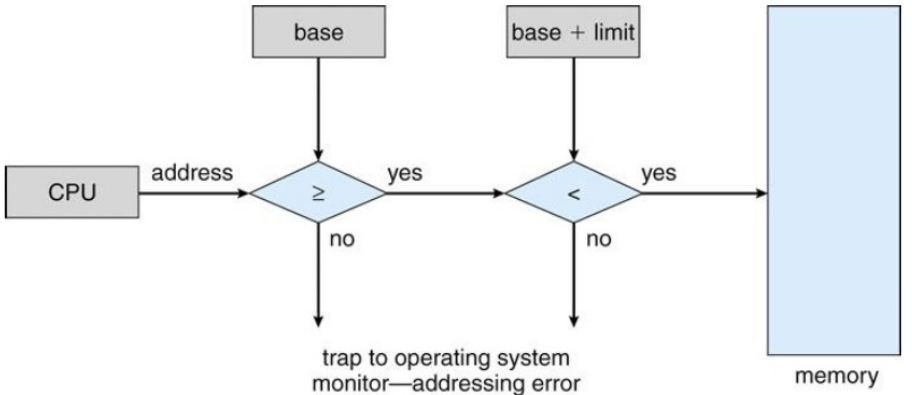
\includegraphics[width=0.33\textwidth]{MMUBaseLimit}\end{figure}

\paragraph{MMU --- Segmentation}
\begin{itemize}
  \item \textbf{Solution} to base + limit: use multiple base + limit register pairs \emph{per process}
  \begin{itemize}
    \item[$ \to $] private + public segments
  \end{itemize}
  \item \textbf{Advantages}:
  \begin{itemize}
    \item[+] data/code sharing between processes possible without compromising confidentiality
    \item[+] process does not need large contiguous physical memory area \( \to \) easy placement
    \item[+] process does not need to be entirely in memory \( \to \) memory overcommitment ok
  \end{itemize}
  \item \textbf{Disadvantages}:
  \begin{itemize}
    \item[-] segments need to be kept contiguous in physical memory
    \item[-] \emph{fragmentation} of physical memory
  \end{itemize}
\end{itemize}

\paragraph{Segmentation --- Architecture}
\begin{itemize}
  \item virtual address = [segment \#, offset]
  \item each process has \emph{segment table}, maps virtual address to physical address in memory
  \begin{itemize}
    \item \emph{base}: starting physical address where segment resides in memory
    \item \emph{limit}: length of segment
    \item \emph{protection}: access restriction (read/write) for safe sharing
  \end{itemize}
  \item MMU has two registers that identify current address space
  \begin{itemize}
    \item \emph{segment-table base register} (STBR): points to segment table location of current process
    \item \emph{segment-table length register} (STLR): indicates number of segments used by process
  \end{itemize}
\end{itemize}
\begin{figure}[h]\centering\label{Segmentation}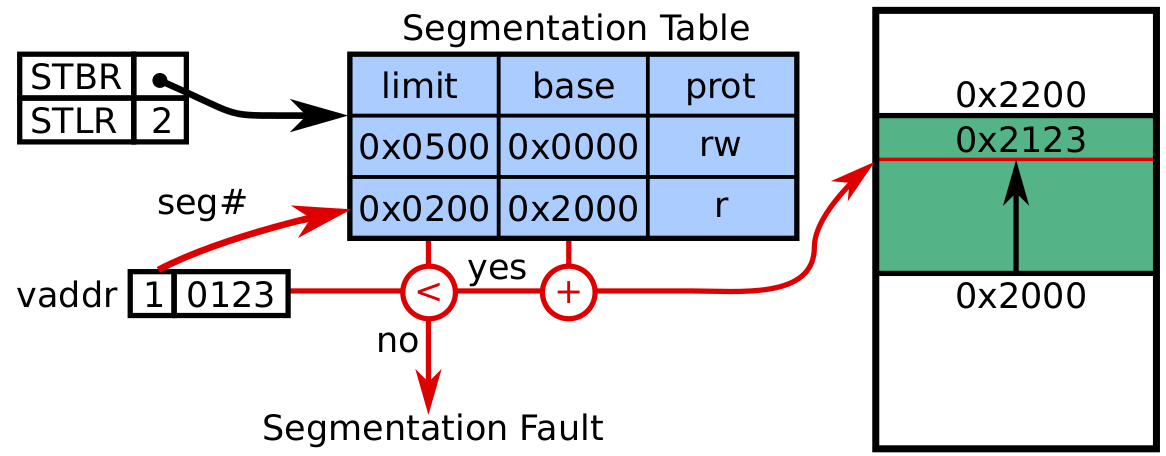
\includegraphics[width=0.33\textwidth]{Segmentation}\end{figure}

\paragraph{External Fragmentation}
\begin{itemize}
  \item \textbf{Fragmentation} = inability to use free memory
  \item \textbf{External Fragmentation} = sum of free memory satisfies requested amount of memory, but is not contiguous
  \item \textbf{Compaction}: reduce external fragmentation
  \begin{itemize}
    \item close gaps by moving allocated memory in one direction
    \item only possible if relocation is dynamic, can be done at execution time
    \item \emph{problem}: expensive! Need to halt process while moving data and updating tables
    \begin{itemize}
      \item[$ \to $] caches need to be reloaded, which should be avoided 
    \end{itemize}
  \end{itemize}
\end{itemize}

\paragraph{MMU --- Paging}
\begin{itemize}
  \item \textbf{Principle}: divide physical memory into fixed-size blocks (\emph{page frames})
  \begin{itemize}
    \item size = \( 2^n \) Bytes (typically 4KiB, 2MiB, 4MiB)
  \end{itemize}
  \item \textbf{Virtual Memory}: divided into same-sized blocks (\emph{pages})
  \item \textbf{Page Table}: managed by OS, stores mappings between \emph{virtual page numbers} (vpn) and \emph{page frame numbers} (pfn) for each AS
  \item OS tracks all free frames, modifies page tables as needed
  \item \textbf{Present Bit} (in page table): indicates that virtual page is currently mapped to physical memory
  \item if process issues instruction to access unmapped virtual address, MMU calls OS to bring in the data (\emph{page fault})
\end{itemize}

\paragraph{MMU --- Address Translation Scheme}
\begin{itemize}
  \item \textbf{Virtual address}: divided into
  \begin{itemize}
    \item \emph{virtual page number}: page table index containing base address of each page in physical memory
    \item \emph{page offset}: concatenated with base address results in physical address
  \end{itemize}
\end{itemize}

\paragraph{MMU --- Hierarchical Page Table}
\begin{itemize}
  \item \textbf{Problem}: need to keep complete page table in memory for every address space
  \item \textbf{Idea}: not needing complete table, most virtual addresses unused by process
  \begin{itemize}
    \item[$ \to $] subdivide virtual address further into multiple page indexes \( p_n \) forming \emph{hierarchical page table}
  \end{itemize}
\end{itemize}

\paragraph{Hierarchical Page Table --- x86-64}
\begin{itemize}
  \item \textbf{long mode}: 4-level hierarchical page table
  \item \textbf{page directory base register} (control register 3, \code{\%CR3}) stores starting physical address of \emph{first level page table}
  \item \textbf{address-space hierarchy}: following page-table hierarchy for every address space:
  \begin{itemize}
    \item page map level 4 (PML4)
    \item page directory pointers table (PDPT)
    \item page directory (PD)
    \item page table entry (PTE)
  \end{itemize}
  \item \textbf{Per level}: table can either point to \emph{directory} in next hierarchy level or to \emph{entry} containing actual mapping data
\end{itemize}
\begin{figure}[h]\centering\label{PageTable}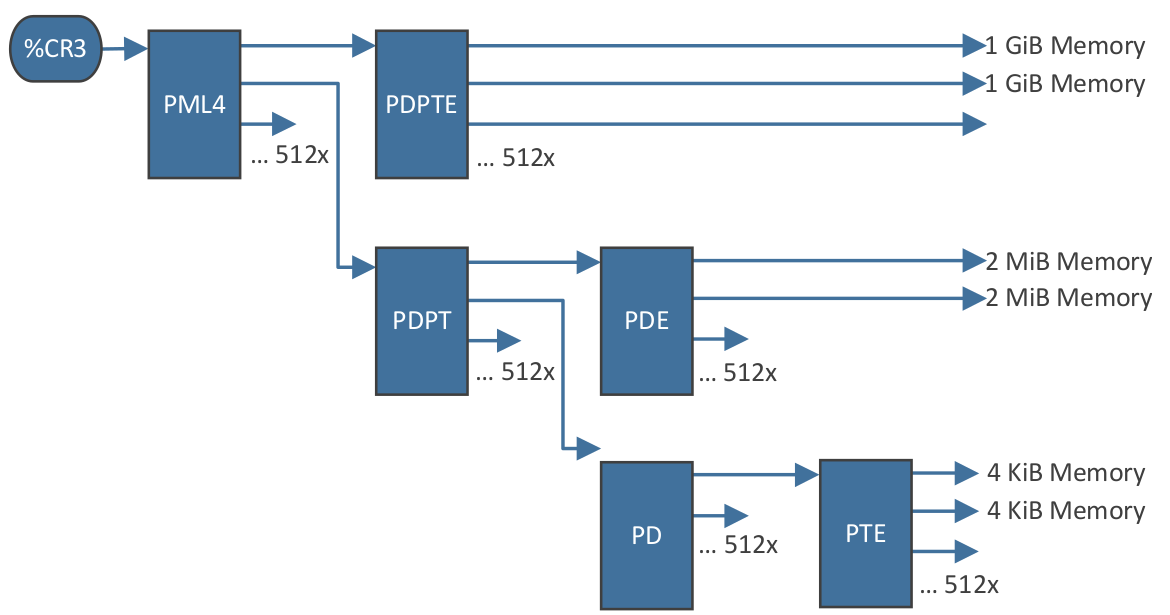
\includegraphics[width=0.33\textwidth]{PageTable}\end{figure}

\paragraph{Page Table Entry --- Content}
\begin{itemize}
  \item \textbf{valid bit} (\emph{present bit}): whether page is currently available in memory or needs to be brought in by OS via \emph{page fault}
  \item \textbf{page frame number}: if page is present: physical address where page is currently located
  \item \textbf{write bit}: whether or not page may be written to (may cause \emph{page fault})
  \item \textbf{caching}: whether or not page should be cached at all (and with which policy)
  \item \textbf{accessed bit}: set by MMU if page was touched since bit was last cleared by OS
  \item \textbf{dirty bit}: set by MMU if page was modified since bit was last cleared by OS
\end{itemize}

\paragraph{Paging --- OS Involvement}
\begin{itemize}
  \item OS performs all operations that require semantic knowledge
  \item \textbf{page allocation} (bringing data into memory): OS needs to find free frame for new pages and set up mapping in page table of affected address space
  \item \textbf{page replacement}: when all page frames are used, OS needs to evict pages from memory
  \item \textbf{context switching}: OS sets MMU's base register (\code{\%CR3} on x86) to point to page hierarchy of next process's address space
\end{itemize}

\paragraph{MMU --- Internal Fragmentation}
\begin{itemize}
  \item \textbf{Paging}: eliminates external fragmentation
  \item \textbf{Problem}: internal fragmentation
  \begin{itemize}
    \item memory can only be allocated in page frame sizes
    \item allocated virtual memory area will generally not end at page boundary
    \item[$ \leadsto $] unused rest of last allocated page is lost!
  \end{itemize}
\end{itemize}

\paragraph{MMU --- Page Size trade-offs}
\begin{itemize}
  \item \textbf{Fragmentation}:
  \begin{itemize}
    \item \emph{larger pages} \( \to \) more memory wasted (internal fragmentation) per allocation
    \item \emph{smaller pages} \( \to \) only half a page wasted per allocation on average
  \end{itemize}
  \item \textbf{Table Size}:
  \begin{itemize}
    \item \emph{larger pages} \( \to \) fewer bits needed for \code{pfn} (more bits in offset), fewer PTEs
    \item \emph{smaller pages} $ \to $ more + larger PTEs
  \end{itemize}
  \item \textbf{I/O}:
  \begin{itemize}
    \item \emph{larger pages} $ \to $ more data needs to be loaded from dist to make page valid
    \item \emph{smaller pages} $ \to $ need to trap OS more often when loading large program
  \end{itemize}
\end{itemize}

\begin{summary}
  \begin{itemize}
    \item need to place processes in memory to run
    \item want to place multiple processes in memory at same time to run concurrently/parallel
    \item \textbf{Virtual Memory}: enables protection, transparency, overcommitment
    \begin{itemize}
      \item emph{trade-off} extra hardware (MMU) to translate addresses at every load/store
    \end{itemize}
    \item \textbf{MMU types}: base + limit, segmentation, paging
    \item \textbf{Paging}: supported by all contemporary MMUs, favorite of most OS
  \end{itemize}
\end{summary}

  % \section{Paging}

\paragraph{Hierarchical Page Table --- two-level page table}
\begin{itemize}
  \item \textbf{Layout}: on 32-bit machine with 4KiB pages divide virtual address into
  \begin{itemize}
    \item \emph{page number} (p): 20 bits
    \item \emph{page offset} (d): 12 bits
  \end{itemize}
  \item \textbf{Table Paging}: table can be paged to save memory -- subdivide vpn:
  \begin{itemize}
    \item index in \emph{page directory} ($ p_1 $): 10 bits
    \item index in \emph{page table entry} ($ p_2 $): 10 bits
  \end{itemize}
  \item for ranges of 1024 invalid pages, reset present bit in page directory
  \begin{itemize}
    \item[$ \to $] save space of second-level page table
  \end{itemize}
\end{itemize}
\begin{figure}[h]\centering\label{TwoLevelPageTable}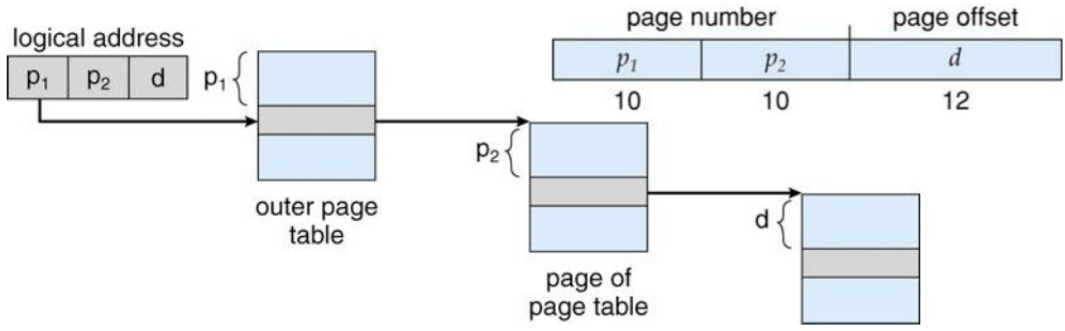
\includegraphics[width=0.33\textwidth]{TwoLevelPageTable}\end{figure}

\paragraph{Linear Inverted Page Table}
\begin{itemize}
  \item \textbf{Problem}: large AS (64 bit) but only few mapped virtual addresses
  \begin{itemize}
    \item[$ \to $] much memory wasted on page tables
    \item[$ \to $] lookup slow due to many levels of hierarchy
  \end{itemize}
  \item \textbf{Idea}: invert page table mapping
  \begin{itemize}
    \item map physical frame to virtual page instead of other way around
    \item single page table for \emph{all processes} (exactly one table per system)
    \item one page table entry for each physical page frame
  \end{itemize}
  \item \textbf{Advantage}: less overhead for page table meta data
  \item \textbf{Disadvantage}: increases time needed to search table when page reference occurs
\end{itemize}
\begin{figure}[h]\centering\label{LinearInvertedPageTable}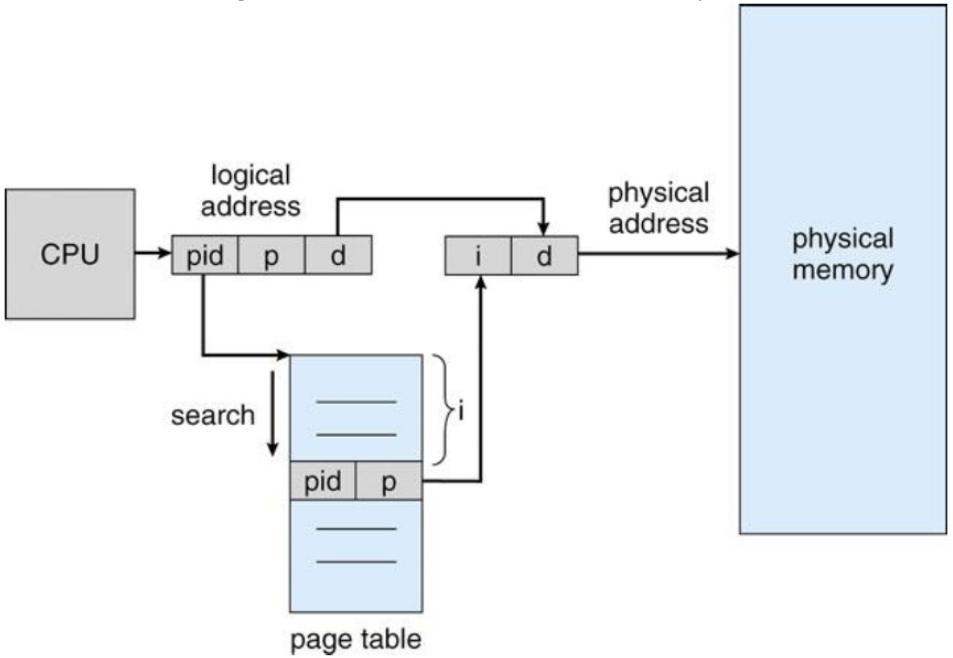
\includegraphics[width=0.33\textwidth]{LinearInvertedPageTable}\end{figure}

\paragraph{Hashed Inverted Page Table}
\begin{itemize}
  \item \textbf{Hash Anchor Table}: limits search to at most a few page-table entries
\end{itemize}

\paragraph{Translation Lookaside Buffer --- Motivation}
\begin{itemize}
  \item \textbf{Naive paging is slow}:
  \begin{itemize}
    \item every load/store requires multiple memory references
    \item 4-level hierarchy: 5 memory references for every load/store (4 page directory/table references, 1 data access)
  \end{itemize}
  \item \textbf{Idea}: add cache that stores recent memory translations
  \begin{itemize}
    \item \emph{translation lookaside buffer} (TLB) maps [vpn] to [pfn, protection]
    \item typically 4-way to fully associative hardware cache in MMU
    \item typically 64-2000 entries
    \item typically 95\%-99\% hit rate
  \end{itemize}
\end{itemize}

\paragraph{TLB --- Operation}
\begin{itemize}
  \item on every load/store:
  \begin{itemize}
    \item check if translation result is cached in TLB (\emph{TLB hit})
    \item otherwise walk page tables, insert result into TLB (\emph{TLB miss})
  \end{itemize}
  \item \textbf{Quick}: can compare many TLB entries in parallel in hardware
\end{itemize}

\paragraph{TLB --- TLB Miss}
\begin{itemize}
  \item \textbf{Process}:
  \begin{itemize}
    \item evict entry from TLB on TLB miss
    \item load entry for missing virtual address into TLB
  \end{itemize}
  \item \textbf{Variants}: \emph{software-managed} and \emph{hardware managed}
  \item \textbf{software-managed TLB}:
  \begin{itemize}
    \item OS receives \emph{TLB miss exception}
    \item OS decides which entry to evict (drop) from TLB
    \item OS generally walks page tables in software to fill new TLB entry
    \item TLB entry format specified in \emph{instruction set architecture} (ISA)
  \end{itemize}
  \item \textbf{hardware-managed TLB}:
  \begin{itemize}
    \item evict TLB entry based on hardware-encoded policy
    \item walk page table in hardware $ \to $ resolve address mapping
  \end{itemize}
\end{itemize}

\paragraph{TLB --- Address Space Identifiers}
\begin{itemize}
  \item \textbf{Problem}: vpn dependent on AS
  \begin{itemize}
    \item vpns in different AS can map to different pfns
    \item[$ \to $] need to clear TLB on AS switch
  \end{itemize}
  \item \textbf{Idea}: solve vpn ambiguity with additional identifiers in TLB
  \item \textbf{ASID}: TLB has \emph{address space identifier} (ASID) in every entry
  \begin{itemize}
    \item map [vpn, ASID] to [pfn, protection]
    \item[$ \to $] avoids TLB flush at every address-space switch
    \item[$ \to $] less TLB misses: some TLB entries still present from last time process ran
  \end{itemize}
\end{itemize}

\paragraph{TLB --- Reach}
\begin{itemize}
  \item[=] amount of memory accessible with TLB hits: $ \text{TLB reach} = \text{TLB size} * \text{page size} $
  \item \textbf{Ideally}: working set of each process is stored in TLB (otherwise high degree of TLB misses)
  \item \textbf{Increase page size}:
  \begin{itemize}
    \item[+] fewer TLB entries per memory needed
    \item[-] increase internal fragmentation
  \end{itemize}
  \item \textbf{multiple page sizes}:
  \begin{itemize}
    \item[+] allows applications that map larger memory areas to increase TLB coverage with minimal fragmentation increase
  \end{itemize}
  \item \textbf{increase TLB size}:
  \begin{itemize}
    \item[-] expensive
  \end{itemize}
\end{itemize}

\paragraph{TLB --- Effective Access Time}
\begin{itemize}
  \item \textbf{Associative lookup}: takes $ \tau $ time units (e.g., $ \tau = 1\text{ns} $)
  \item \textbf{Memory cycle}: takes $ \mu $ time units (e.g., $ \mu = 100\text{ns} $)
  \item \textbf{TLB hit ratio} $ \alpha $: percentage of all memory accesses with cached translation (e.g., $ \alpha = 99\% $)
  \item \textbf{Effective Access Time} (EAT) for linear page table without cache:
    \begin{equation*}
      \text{EAT} = (\tau + \mu)\alpha + (\tau + 2\mu)(1-\alpha) = \tau + 2\mu - \mu\alpha
    \end{equation*}
\end{itemize}

\begin{summary}
  \begin{itemize}
    \item page tables communicate between OS and MMU hardware
    \begin{itemize}
      \item how virtual addresses in each address space translate to physical addresses
      \item which kind of accesses the MMU should allow/signal to the OS
    \end{itemize}
    \item different page table layouts have been developed
    \begin{itemize}
      \item linear page table
      \item hierarchical page tables
      \item inverted page tables
      \item hashed page tables
    \end{itemize}
    \item performing page table lookups for every memory access significantly slows down execution time of programs
    \begin{itemize}
      \item translation lookaside buffer (TLB) caches previously performed page table lookups
      \item typical TLBs cover $ 95\%-99\% $ of all translations
    \end{itemize}
  \end{itemize}
\end{summary}

  % \section{Caching}

\paragraph{Caching --- Motivation}
\begin{itemize}
  \item memory (RAM) needs to be managed carefully
  \item \textbf{Ideal} properties: large, fast, nonvolatile, cheap
  \item \textbf{Real} memory: trade-offs
\end{itemize}

\paragraph{Caching --- Cache misses}
\begin{itemize}
  \item \textbf{Compulsory miss}:
  \begin{itemize}
    \item cold start, first reference
    \item data block was not cached before
  \end{itemize}
  \item \textbf{Capacity miss}:
  \begin{itemize}
    \item not all required data fits into cache
    \item accessed data previously evicted to make room for different data
  \end{itemize}
  \item \textbf{Conflict miss}:
  \begin{itemize}
    \item collision, interference
    \item depending on cache organization, data items interfere with each other
    \item fully associative caches are not prone to conflict misses
  \end{itemize}
\end{itemize}

\paragraph{Caching --- Harvard architecture}
\begin{itemize}
  \item \textbf{Principle}: separate buffer memory for data and instructions
\end{itemize}
\begin{figure}[h]\centering\label{CachingHarvard}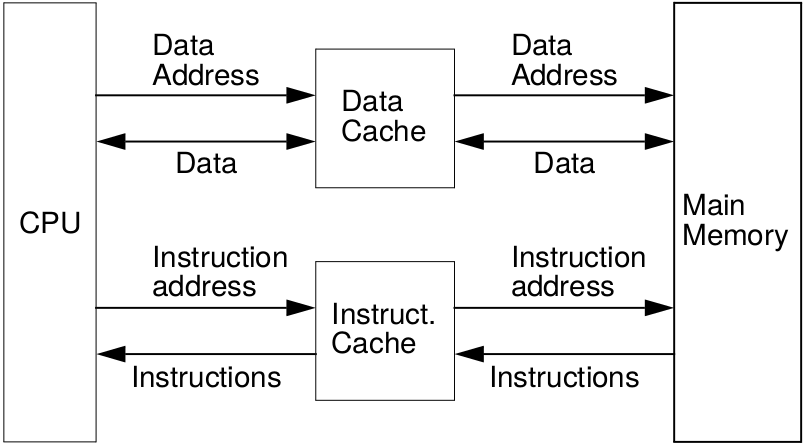
\includegraphics[width=0.33\textwidth]{CachingHarvard}\end{figure}

\paragraph{Caching --- write/replacement policies}
\begin{itemize}
  \item \textbf{Cache hit}:
  \begin{itemize}
    \item \emph{write-through}: main memory always up-to-date, writes might be slow
    \item \emph{write-back}: data written only to cache, main memory temporarily inconsistent
  \end{itemize}
  \item \textbf{Cache miss}:
  \begin{itemize}
    \item \emph{write-allocate}: data read from main memory to cache, write performed afterwards
    \item \emph{write-to-memory}: modification is performed only in main memory
  \end{itemize}
\end{itemize}

\paragraph{Cache Design Parameters}
\begin{itemize}
  \item \textbf{Size + Set size}: small cache $ \to $ set-associative implementation with large sets
  \item \textbf{Line length}: spatial locality $ \to $ long cache lines
  \item \textbf{Write policy}: temporal locality $ \to $ write-back
  \item \textbf{Replacement policy}
  \item \textbf{Tagging/Indexing}: virtual or physical addresses
\end{itemize}

\paragraph{Caching --- Problems}
\begin{itemize}
  \item \textbf{Ambiguity problem}: same virtual addresses point to different physical addresses at different times
  \item \textbf{Alias problem}: different virtual addresses point to same physical memory location
\end{itemize}

\paragraph{Caching --- virtually indexed, virtually tagged}
\begin{itemize}
  \item \textbf{Operations}:
  \begin{itemize}
    \item \emph{context switch}: cache must be invalidated (and written back if write-back is used)
    \item \emph{fork}: child needs complete copy of parent's address space
    \item \emph{exec}: invalidate cache, no write-back necessary
    \item \emph{exit}: flush cache
    \item \emph{brk/sbrk}: growing = nothing, shrinking = (selective) cache invalidations
  \end{itemize}
  \item \textbf{shared memory/memory-mapped files}: alias problem!
  \begin{itemize}
    \item disallow, do not cache
    \item only allow addresses mapping to same cache line (if using direct-mapped write-allocate cache)
    \item each frame accessible from exactly one virtual address at any time $ \to $ alias page invalidation
  \end{itemize}
  \item \textbf{I/O}:
  \begin{itemize}
    \item \emph{buffered I/O}: no problems 
    \item \emph{unbuffered I/O}:
    \begin{itemize}
      \item write: information may still be in cache $ \to $ write back before I/O starts
      \item read: cache must be invalidated
    \end{itemize}
  \end{itemize}
\end{itemize}
\begin{figure}[h]\centering\label{VIVT}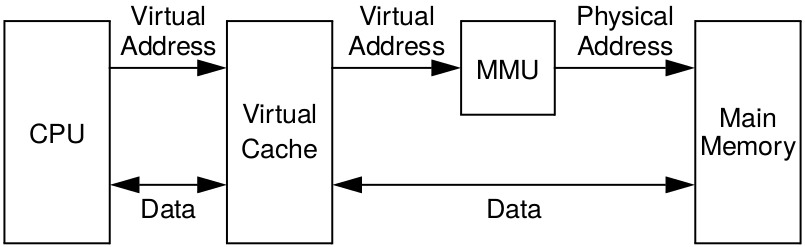
\includegraphics[width=0.33\textwidth]{VIVT}\end{figure}

\paragraph{Caching --- virtually indexed, physically tagged}
\begin{itemize}
  \item \textbf{Usage}: often used as first-level cache
  \item \textbf{Management}:
  \begin{itemize}
    \item no ambiguities
    \item no cache flush/context switch
    \item shared memory/memory mapped files: virtual starting addresses must be mapped to same cache line
    \item I/O: cache flush required
  \end{itemize}
  \item \textbf{Conflicts}: data structures with address distance = multiple of cache size are mapped to same line
  \item \textbf{Runtime properties}:
  \begin{itemize}
    \item \emph{cache flush}: avoidable most times (fast context switches, interrupt-handling, syscalls)
    \item \emph{deferred write-back after context switch}:
    \begin{itemize}
      \item avoids write accesses $ \to $ performance gain
      \item variable execution time caused by compulsory misses
    \end{itemize}
    \item \emph{dynamic memory management}: causes variable execution times through conflict misses
    \item \emph{multiprocessor systems}: problematic with shared memory --- which line should be invalidated?
    \begin{itemize}
      \item cache size is small multiple of page size (1-4)
      \item requires to only invalidate/flush 1-4 cache lines by cache coherency HW
    \end{itemize}
  \end{itemize}
\end{itemize}
\begin{figure}[h]\centering\label{VIPT}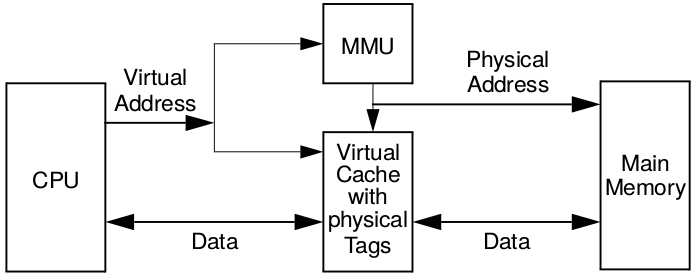
\includegraphics[width=0.33\textwidth]{VIPT}\end{figure}

\paragraph{Caching --- physically indexed, physically tagged}
\begin{itemize}
  \item \textbf{Advantages}:
  \begin{itemize}
    \item[+] completely transparent to processor
    \item[+] no performance-critical system support required (including I/O)
    \item[+] SMPs with shared memory can use coherency protocol implemented in hardware
  \end{itemize}
  \item \textbf{random allocation conflicts}:
  \begin{itemize}
    \item page conflicts caused by random allocation of physical memory
    \item contiguous virtual memory normally mapped to arbitrary free physical pages
  \end{itemize}
  \item \textbf{random coloring conflicts}: consequences of random page coloring:
  \begin{itemize}
    \item cache conflicts
    \item cache only partially used
    \item significant runtime variations
  \end{itemize}
  \item \textbf{conflict mitigation}:
  \begin{itemize}
    \item sequential page colors for individual memory segments
    \item \emph{cache partitioning}: divide physical memory in disjoint subsets, all pages of subset are mapped to same cache partition
  \end{itemize}
\end{itemize}
\begin{figure}[h]\centering\label{PIPT}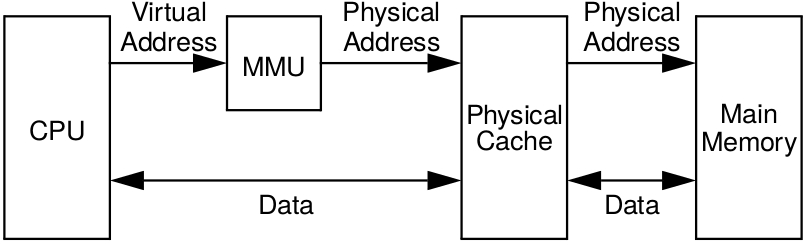
\includegraphics[width=0.33\textwidth]{PIPT}\end{figure}

  % \section{Page Faults}

\paragraph{Page Faults --- handling}
\begin{items}
  \item \textbf{Cause}: access to page currently not present in main memory \\*
    $ \to $ exception, invoking OS
  \item \textbf{Process}: \\*
    $ - $ OS checks access validity (requiring additional info) \\*
    $ - $ get empty frame \\*
    $ - $ load contents of requested page from disk into frame \\*
    $ - $ adapt page table \\*
    $ - $ set present bit of respective entry \\*
    $ - $ restart instruction causing page fault
\end{items}

\paragraph{Page Faults --- latency}
\begin{items}
  \item \textbf{fault rate} $ 0 \leq p \leq 1 $ \\*
    $ - $ $ p = 0 $: no page faults \\*
    $ - $ $ p = 1 $: every reference leads to page fault
  \item \textbf{effective access time} (EAT): \\*
    $ \text{EAT} = (1-p)*\text{memory access} + p*(\text{PF overhead} + \text{PF service time} + \text{restart overhead}) $
\end{items}

\paragraph{Page Faults --- performance impact}
\begin{items}
  \item \textbf{memory access time}: 200ns
  \item \textbf{average page fault service time}: 8ms
  \item $ \leadsto $ 1:1000 access-page-fault-rate $ \to $ $ \text{EAT} = 8.2\mu s $ $ \Rightarrow $ \emph{slowdown by factor 40}!
\end{items}

\paragraph{Page Faults --- challenges}
\begin{items}
  \item \textbf{what to eject?} \\*
    $ - $ how to allocate frames among processes? \\*
    $ - $ which particular process's pages to keep in memory? \\*
    $ - $ see \emph{page frame allocation}
  \item \textbf{what to fetch?} \\*
    $ - $ what if block size $ \neq $ page size? \\*
    $ - $ just one page needed? prefetch more?
  \item \textbf{process resumption?} \\*
    $ - $ need to save state + resume \\*
    $ - $ process might have been in middle of instruction
\end{items}

\paragraph{Page Faults --- what to fetch?}
\begin{items}
  \item bring in page causing fault
  \item \textbf{pre-fetch} sourrounding pages? \\*
    $ - $ reading two disk blocks is approximately as fast as reading one \\*
    $ - $ as long as there is no track/head switch, seek (disk) time dominates \\*
    $ - $ application exhibits spatial locality = big win
  \item \textbf{pre-zero} pages? \\*
    $ - $ don't want to leak information between processes \\*
    $ - $ need 0-filled pages for stack, heap, .bss, \dots \\*
    $ - $ \emph{zero on demand}? \\*
    $ - $ keep pool of 0-pages filled in background when CPU is idle?
\end{items}

\paragraph{Page Faults --- process resumption?}
\begin{items}
  \item hardware provides info about page fault \\*
    (intel: \code{\%cr2} contains faulting virtual address)
  \item \textbf{context}: OS needs to figure out fault context: \\*
    $ - $ read or write? \\*
    $ - $ instruction fetch? \\*
    $ - $ user access to kernel memory?
  \item \textbf{idempotent instructions}: easy: \\*
    $ - $ re-do load/store instructions \\*
    $ - $ re-execute instructions accessing only one address
  \item \textbf{complex instructions}: must be re-started \\*
    $ - $ some CISC instructions are hard to restart (e.g., block move of overlapping areas) \\*
    $ - $ \emph{solutions}: \\*
      \phantom{$ - $} $ \cdot $ touch relevant pages before operation starts \\*
      \phantom{$ - $} $ \cdot $ keep modified data in registers $ \to $ page faults can't take place \\*
      \phantom{$ - $} $ \cdot $ design ISA such that complex operations can execute partially $ \to $ consistent page fault state
\end{items}

\paragraph{Memory-Mapped Files --- other issues}
\begin{items}
  \item \textbf{I/O mapping}: mapping disk block to page in memory allows file I/O to be treated as routing memory  \\*
    $ - $ \emph{initial}: read page-sized portion of file from file system to physical page \\*
    $ - $ \emph{subsequent read/write}: treated as ordinary memory access \\*
    $ \to $ \emph{simplifies} file access, file I/O through memory instead of syscalls \\*
    $ \to $ \emph{memory-file sharing}: several processes can map to same file
\end{items}

\paragraph{Shared Data Segments}
\begin{items}
  \item \textbf{implementation}: \\*
    $ - $ temporary, asynchronous memory-mapped files \\*
    $ - $ shared pages (with allocated space on backing store)
  \item \textbf{copy on write} (COW): \\*
    $ - $ allows both parent and child process to initially share same memory pages \\*
    $ - $ only modified pages are copied $ \to $ more efficient process creation
\end{items}

\paragraph{Page Frame Allocation --- local vs. global}
\begin{items}
  \item \textbf{global}: all frames considered for replacement \\*
    $ - $ does not consider page ownership \\*
    $ - $ one process cannot get another process's frame \\*
    $ - $ does not protect process from a process that hogs all memory
  \item \textbf{local}: only frames of faulting process are considered for replacement \\*
    $ - $ isolates processes/users \\*
    $ - $ separately determine how many frames each process gets
\end{items}

\paragraph{Fixed Allocation --- equal vs. proportional}
\begin{items}
  \item \textbf{equal}: all processes get same amount of frames
  \item \textbf{proportional}: allocate according to process size \\*
    $ s_i \coloneqq \text{size of process } p_i $, $ S \coloneqq \sum s_i $, $ m \coloneqq \text{total number of frames } $ \\*
    $ \Rightarrow a_i \coloneqq \frac{s_i}{S}m $ allocation for $ p_i $
\end{items}

\paragraph{Fixed Allocation --- priority allocation}
\begin{items}
  \item = proportional allocation scheme using priorities rather than size
  \item \textbf{on page fault} of $ P_i $: \\*
    $ - $ select one of its frames for replacement or \\*
    $ - $ select frame from process with lower priority
\end{items}

\paragraph{Memory Locality}
\begin{items}
  \item \textbf{problem}: background storage much slower than memory \\*
    $ - $ paging extends memory size using background storage \\*
    $ - $ \emph{goal}: run near memory speed, not near background storage speed
  \item \textbf{Pareto principle}: applies to working sets of processes \\*
    $ - $ 10\% of memory gets 90\% of references \\*
    $ - $ \emph{goal}: keep those 10\% in memory, rest on disk \\*
    $ - $ \emph{problem}: how to identify those 10\%?
\end{items}

\paragraph{Thrashing}
\begin{items}
  \item \textbf{problem}: system is busy swapping pages in and out \\*
    $ - $ each time one page is brought in, another page, whose contents will soon matter, is thrown out \\*
    $ - $ \emph{effect}: low CPU utilization, processes wait for pages to be fetched from disk \\*
    $ - $ \emph{consequence}: OS thinks that it needs higher degree of multiprogramming
  \item \textbf{reasons}: \\*
    $ - $ \emph{no temporal locality} of access pattern --- process doesn't follow Pareto principle \\*
    $ - $ \emph{too much multiprogramming}: each process fits individually, but too many for system \\*
    $ - $ \emph{memory too small} to hold hot memory of a single process (the 10\%) \\*
    $ - $ \emph{bad page replacement policy}
\end{items}

\paragraph{Working-Set Model}
\begin{items}
  \item $ \Delta \coloneqq $ working-set window (fixed number of page references; e.g., 10000 instructions)
  \item $ \text{WSS}_i \coloneqq $ working set of process $ P_i $ \\*
    $ - $ total number of pages referenced in most recent $ \Delta $ (varies in time) \\*
    $ - $ $ \Delta \begin{cases}
      \text{too small} &\Rightarrow \text{ will not encompass entire locality} \\
      \text{too large} &\Rightarrow \text{ will encompass several localities} \\
      = \infty &\Rightarrow \text{ will encompass entire program}
    \end{cases} $
  \item $ D \coloneqq \sum \text{WSS}_i = $ total demand for frames \\*
    $ - $ $ D > m \leadsto $ \textbf{thrashing} \\*
    $ \to $ $ D > m \Rightarrow $ suspend a process
\end{items}

\paragraph{Working Set --- keeping track}
\begin{items}
  \item \textbf{perfect}: replace page that is referenced furthest in the future (\emph{oracle})
  \item \textbf{idea}: predict future from past \\*
    $ - $ record page references from past and extrapolate into future \\*
    $ - $ \emph{problem}: too expensive to make ordered list of all page references at runtime
  \item \textbf{idea}: sacrifice precision for speed \\*
    $ - $ MMU sets \emph{reference bit} in respective page table entry every time a page is referenced \\*
    $ - $ set timer to scan all page table entries for reference bits
\end{items}

\paragraph{Page Fault Frequency --- allocation scheme}
\begin{items}
  \item \textbf{goal}: establish acceptable page fault rate \\*
    $ - $ \emph{actual rate too low} $ \to $ give frames to other process \\*
    $ - $ \emph{actual rate too high} $ \to $ allocate more frames to process
\end{items}

\paragraph{Page Fetch Policy --- demand paging}
\begin{items}
  \item \textbf{idea}: only transfer pages raising page faults
  \item \textbf{advantages}: \\*
    $ - $ only transfer what is needed \\*
    $ - $ less memory needed by process $ \to $ higher multiprogramming degree possible
  \item \textbf{disadvantages}: \\*
    $ - $ many initial page faults when task starts \\*
    $ - $ more I/O operations $ \to $ more I/O overhead
\end{items}

\paragraph{Page Fetch Policy --- pre-paging}
\begin{items}
  \item \textbf{idea}: speculatively transfer pages to RAM \\*
    $ - $ at every page fault: speculate what else should be loaded \\*
    $ - $ e.g., load entire text section when process starts
  \item \textbf{advantage}: improves disk I/O throughput
  \item \textbf{disadvantages}: \\*
    $ - $ wastes I/O bandwidth if page is never used \\*
    $ - $ can destroy working set of other processes in case of page stealing
\end{items}

\begin{summary}
  \begin{items}
    \item paging simulates a memory size of the size of the virtual memory
    \item when pages are filled via page faults, OS needs to answer some questions: \\*
      $ - $ what to eject? \\*
      $ - $ what to fetch? \\*
      $ - $ how to resume process?
    \item different strategies to allocate frames and replace pages: \\*
      $ - $ local vs. global allocation \\*
      $ - $ fixed vs. proportional vs. priority allocation
    \item \emph{thrashing} must be prevented by taking working sets of active processes into account
  \end{items}
\end{summary}

  % \section{Page Replacement Policies}

\paragraph{Page Replacement --- naive}
\begin{itemize}
  \item \textbf{step 1: save/clear victim page}: \\*
    $ - $ drop page if fetched from disk and clean \\*
    $ - $ \emph{dirty}: write back modifications if from disk and dirty (unless \code{MAP_COPY}) \\*
    $ - $ \emph{non-dirty}: write page file/swap partition otherwise (e.g., stack, heap memory)
  \item \textbf{step 2: unmap page from old AS}: invalidate PTE, flush cache
  \item \textbf{step 3: prepare new page}: null page or load new contents
  \item \textbf{step 4: map page frame into new AS}: invalidate PTE, flush cache
\end{itemize}

\paragraph{Page Replacement --- buffering}
\begin{itemize}
  \item \textbf{problem}: naive page replacement encompasses two I/O transfers \\*
    $ \to $ both operations block page fault from completing
  \item \textbf{goal}: reduce I/O from critical page fault path to speed up page faults
  \item \textbf{idea}: keep pool of free page frames (\emph{pre-cleaning}): \\*
    $ - $ \emph{on page fault}: use page frame from free pool \\*
    $ - $ \emph{cleaning}: daemon cleans, reclaims and scrubs pages for free pool in background \\*
    $ \to $ smooths out I/O, speeds up paging significantly
  \item \textbf{remaining problem}: which pages to select as victims? \\*
    $ - $ \emph{goal}: identify page that has left working set of its processes, add to free pool \\*
    $ - $ \emph{success metric}: low overall page fault rate
\end{itemize}

\paragraph{Page Replacement --- FIFO}
\begin{itemize}
  \item \textbf{idea}: evict oldest fetched page in system
  \item \textbf{Belady's Anomaly}: using FIFO, for every number $ n $ of page frames you can construct a reference string that performs worse with $ n+1 $ frames \\*
  $ \to $ with FIFO it is possible to get more page faults with more page frames!
\end{itemize}

\paragraph{Page Replacement --- oracle}
\begin{itemize}
  \item = optimal replacement strategy: replace page whose next reference is furthest in future
  \item \textbf{problem}: future unpredictable
  \item \textbf{however}: good metric to check how well other algorithms perform
\end{itemize}

\paragraph{Page Replacement --- LRU}
\begin{itemize}
  \item \textbf{goal}: approximate oracle page replacement
  \item \textbf{idea}: past often predicts future well
  \item \textbf{assumption}: page used furthest in past is used furthest in future
  \item \textbf{cycle counter implementation}: \\*
    $ - $ have MMU write CPU's time stamp counter to PTE on every access \\*
    $ - $ \emph{page fault}: scan all PTEs to find oldest counter value \\*
    $ - $ \emph{advantage}: cheap at access if done in HW \\*
    $ - $ \emph{disadvantage}: memory traffic for scanning
  \item \textbf{stack implementation}: \\*
    $ - $ keep doubly linked list of all page frames \\*
    $ - $ move each referenced page to tail of list \\*
    $ - $ \emph{advantage}: can find replacement victim in $ O(1) $ \\*
    $ - $ \emph{disadvantage}: need to change 6 pointers at every access
  \item $ \leadsto $ \textbf{no silver bullet}: \\*
    $ - $ \emph{observation}: predicting future based on past is not precise \\*
    $ - $ \emph{conclusion}: relax requirements --- maybe perfect LRU isn't needed? $ \Rightarrow $ approximate LRU
\end{itemize}

\paragraph{LRU Approximation --- clock page replacement}
\begin{itemize}
  \item aka \emph{second chance page replacement}
  \item \textbf{precondition}: MMU sets reference bit in PTE \\*
    $ - $ supported natively by most hardware \\*
    $ - $ can easily emulate in systems with software managed TLB (e.g., MIPS)
  \item \textbf{store}: keep all pages in circular FIFO list
  \item \textbf{searching} for victim: scan pages in FIFO's order \\*
    $ - $ if reference bit = 0 $ \to $ use page as victim and advance \\*
    $ - $ if reference bit = 1 $ \to $ set to 0, continue scanning
  \item \textbf{problem}: large memory $ \to $ most pages referenced before scanned \\*
    $ - $ \emph{solution}: use 2 arms, leading arm clears reference bit, trailing arm selects victim
\end{itemize}

\paragraph{Replacement Strategies --- other}
\begin{itemize}
  \item \textbf{random eviction}: pick random victim \\*
    $ - $ dirt simple \\*
    $ - $ not overly horrible in reality
  \item \textbf{larger counter}: use $ n $-bit reference counter instead of reference bit \\*
    $ - $ \emph{least frequently used}: rarely used page not in a working set $ \to $ replace page with smallest count \\*
    $ - $ \emph{most frequently used}: page with smallest count probably just brought in $ \to $ replace page with \\* \phantom{$ - $} \phantom{$ \cdot $} largest count \\*
    $ - $ neither LFU nor MDU are common (no such hardware, not that great)
\end{itemize}

\begin{summary}
  \begin{itemize}
    \item victim page frame needs to be selected by OS when handling page faults \\*
      $ - $ evicting page frame after page fault happens = not a good idea \\*
      $ - $ page buffering keeps eviction out of critical path
    \item different victim selection policies exist \\*
      $ - $ FIFO $ \to $ Belady's Anomaly \\*
      $ - $ Oracle $ \to $ cannot predict the future \\*
      $ - $ Random $ \to $ unpredictable, never great but rarely very bad \\*
      $ - $ LRU $ \to $ hard to implement efficiently
  \end{itemize}
\end{summary}

  % \section{Memory Allocation}

\paragraph{Memory Allocation --- dynamic}
\begin{items}
  \item = allocate + free memory chunks of arbitrary size at arbitrary points in time \\*
    $ - $ almost every program uses it (heap) \\*
    $ - $ don't have to statically specify complex data structures \\*
    $ - $ can have data grow as function of input size \\*
    $ - $ kernel itself uses dynamic memory allocation for its data structures
  \item \textbf{implementation}: has huge impact on performance, both in user and kernel space
  \item \textbf{fact}: it is impossible to construct memory allocator that always performs well \\*
    $ \to $ need to understand trade-offs to pick good allocation strategy
\end{items}

\paragraph{Dynamic Memory Allocation --- principle}
\begin{items}
  \item \textbf{initial}: pool of free memory
  \item \textbf{tasks}: \\*
    $ - $ satisfy arbitrary \code{allocate} + \code{free} requests from pool \\*
    $ - $ track which parts are in use/are free
  \item \textbf{restrictions}: \\*
    $ - $ cannot control order/number of requests \\*
    $ - $ cannot move allocated regions $ \to $ fragmentation = core problem!
\end{items}

\paragraph{Dynamic Memory Allocation --- bitmap}
\begin{items}
  \item \textbf{idea}: \\*
    $ - $ divide memory in allocation units of fixed size \\*
    $ - $ use bitmap to keep track if allocated (1) or free (0)
  \item \textbf{problem}: needs additional data structure to store allocation length (otherwise cannot infer whether two adjacent allocations belong together or not from bitmap)
\end{items}

\paragraph{Dynamic Memory Allocation --- list}
\begin{items}
  \item \textbf{method 1}: use one list-node for each allocated data \\*
    $ - $ \emph{extra space} needed for list \\*
    $ - $ allocation lengths already stored
  \item \textbf{method 2}: use one list-node for each unallocated data \\*
    $ - $ can keep list in unallocated area (store size of free area + pointer to next free area in free area) \\*
    $ - $ \emph{additional data structure} needed to store allocation lengths \\*
    $ - $ can search for free space with low overhead
  \item \textbf{method 3}: both
\end{items}

\paragraph{Dynamic Memory Allocation --- problems}
\begin{items}
  \item \textbf{fragmentation} is hard to handle
  \item \textbf{factors} needed for fragmentation to occur: \\*
    $ - $ \emph{different lifetimes} \\*
    $ - $ \emph{different sizes} \\*
    $ - $ \emph{inability to relocate previous allocations}
  \item all fragmentation factors present in dynamic memory allocators!
\end{items}

\paragraph{Allocation --- best fit vs. worst fit}
\begin{items}
  \item \textbf{idea}: keep large free memory chunks together for larger allocation requests that may arrive later
  \item \textbf{best-fit}: allocate smallest free block large enough to store allocation request \\*
    $ - $ must search entire list \\*
    $ - $ \emph{problem}: sawdust --- remainder so small that over time left with unusable sawdust everywhere \\*
    $ - $ \emph{idea}: minimize sawdust by turning strategy around
  \item \textbf{worst-fit}: allocate largest free block \\*
    $ - $ must search entire list \\*
    $ - $ \emph{reality}: worse fragmentation than best-fit
\end{items}

\paragraph{Allocation --- first fit}
\begin{items}
  \item \textbf{idea}: if fragmentation occurs with best and worst fit, optimize for allocation speed
  \item \textbf{principle}: allocate first hole big enough \\*
    $ - $ fastest allocation policy \\*
    $ - $ produced leftover holes of variable size \\*
    $ - $ \emph{reality}: almost as good as best-fit
\end{items}

\paragraph{First Fit --- variants}
\begin{items}
  \item \textbf{first-fit sorted by address order}
  \item \textbf{LIFO first-fit}
  \item \textbf{next fit}
\end{items}

\paragraph{Allocation --- buddy allocator}
\begin{items}
  \item \textbf{idea}: allocate memory in powers of 2 \\*
    $ - $ all chunks have fixed $ 2^n $-size $ \to $ allocation request rounded up to next-higher power of 2 \\*
    $ - $ all chunks naturally aligned
  \item \textbf{no sufficiently small block available}: \\*
    $ - $ select larger available chunk, split into two same-sized buddies \\*
    $ - $ continue until appropriately sized chunk is available
  \item \textbf{two buddies both free} ($ 2^n $): merge to $ 2^{n+1} $-chunk
\end{items}

\paragraph{Real Program Patterns}
\begin{items}
  \item \textbf{ramps}: accumulate data monotonically over time
  \itm \textbf{peaks}: allocate many objects, use briefly, then free all
  \item \textbf{plateaus}: allocate many objects, use for long time
\end{items}

\paragraph{Allocation --- slabs}
\begin{items}
  \item kernel often allocates/frees memory for few, specific data objects of fixed size
  \item \textbf{slab}: multiple pages of contiguous physical memory \\*
    $ - $ linux: uses buddy allocator as underlying allocator for slabs
  \item \textbf{cache}: one or multiple slabs \\*
    $ - $ stores only one kind of object (fixed size)
\end{items}

\begin{summary}
  \begin{items}
    \item dynamic memory means allocating and freeing memory chunks of different sizes at any time
    \item impossible to construct memory allocator that always performs well
    \item typical dynamic memory data structures: \\*
      $ - $ bitmaps \\*
      $ - $ lists
    \item simple, well-performing allocation strategies: \\*
      $ - $ best-fit \\*
      $ - $ first-fit
    \item advanced strategies: \\*
      $ - $ buddy-allocator \\*
      $ - $ slab-allocator
  \end{items}
\end{summary}

  % \section{Secondary Storage}

\paragraph{Secondary Storage --- Structure}
\begin{itemize}
  \item hard disk drives
  \item solid state drive
  \item RAID structure
  \item tertiary storage devices (DVD, magnetic tape)
\end{itemize}

\paragraph{Hard Disk Drives --- Anatomy}
\begin{itemize}
  \item stack of magnetic platters
  \item disk arms contain disk heads per recording surface, read/write to platters
  \item \textbf{Storage}:
  \begin{itemize}
    \item platters divided into concentric \emph{tracks}
    \item \emph{cylinder}: stack of tracks of fixed radius
    \item tracks of fixed radius divided into \emph{sectors}
  \end{itemize}
\end{itemize}

\paragraph{Flash Memory}
\begin{itemize}
  \item \textbf{advantages}:
  \begin{itemize}
    \item[+] solid state
    \item[+] lower power consumption/heat
    \item[+] no mechanical seek 
  \end{itemize}
  \item \textbf{disadvantages}:
  \begin{itemize}
    \item[-] limited number of overwrites
    \item[-] limited durability 
  \end{itemize}
\end{itemize}

\paragraph{RAID}
\begin{itemize}
  \item \textbf{Idea}: improve performance/reliability of storage system by storing redundant data
\end{itemize}
\begin{figure}[h]\centering\label{RAID}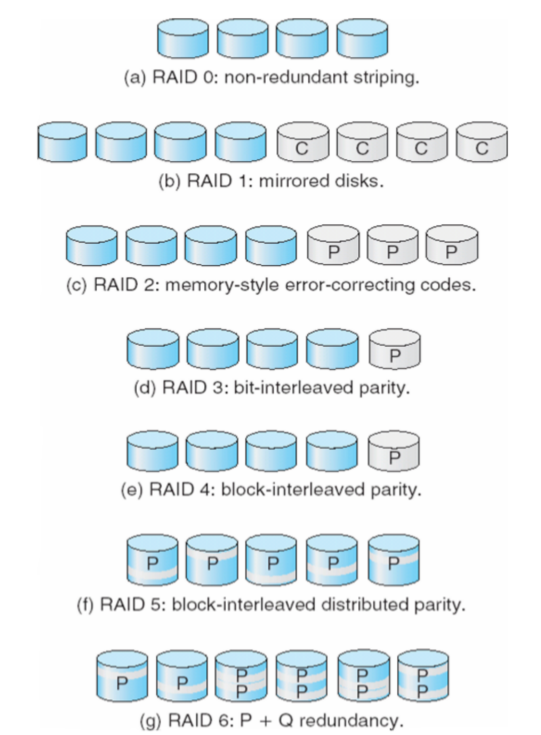
\includegraphics[width=0.2\textwidth]{RAID}\end{figure}

  % \section{File Systems}

\paragraph{File Systems --- motivation}
\begin{itemize}
  \item \textbf{goal}: enable storing of large data amounts \\*
    $ - $ store data/program consistently + persistently \\*
    $ - $ easily look up previously stored data/program
  \item \textbf{file types}: \\*
    $ - $ \emph{data} (numeric, character, binary) \\*
    $ - $ \emph{program}
\end{itemize}

\paragraph{File Systems --- overview}
\begin{itemize}
  \item OS may support multiple file systems
  \item \textbf{namespace}: all file systems typically bound into single namespace (often hierarchical, rooted tree)
\end{itemize}

\paragraph{Files -- abstract operations}
\begin{itemize}
  \item \textbf{file}: abstract data type/object, offering \\*
    $ - $ \code{create}, \code{write}, \code{read}, \\*
    $ - $ \code{reposition} (within file), \\*
    $ - $ \code{delete}, \code{truncate}, \\*
    $ - $ \code{open(}$ F_i $\code{)} (search directory structure on disk for entry $ F_i $, move meta data to memory),  \\*
    $ - $ \code{close(}$ F_i $\code{)} (move cached meta data of entry $ F_i $ in memory to directory structure on disk)
\end{itemize}
\begin{figure}[h]\centering\label{FileSystemInteraction}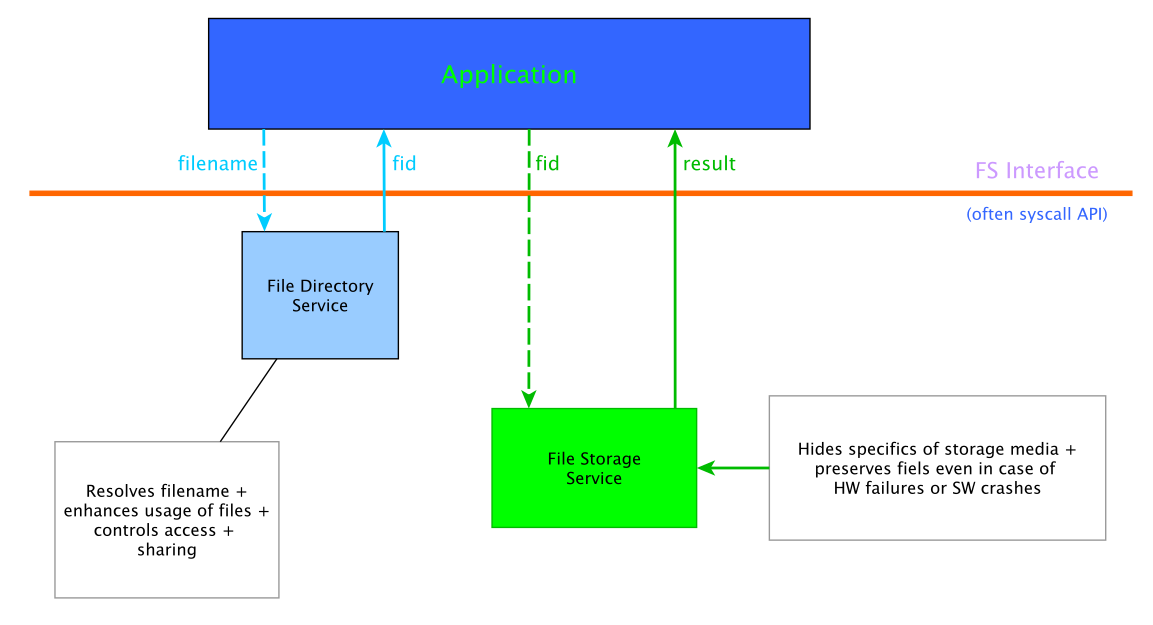
\includegraphics[width=0.4\textwidth]{FileSystemInteraction}\end{figure}

\paragraph{File Management --- goals}
\begin{itemize}
  \item provide convenient file naming scheme
  \item provide uniform I/O support for variety of storage device types
  \item provide standardized set of I/O interface functions
  \item minimize/eliminate loss/corruption of data
  \item provide I/O support + access control for multiple users
  \item enhance system administration (e.g., backup)
  \item provide acceptable performance
\end{itemize}

\paragraph{File Management --- open files}
\begin{itemize}
  \item several meta data is needed to manage open files
  \item \textbf{file pointer}: pointer to last read/write location, per process that has file opened
  \item \textbf{access rights}: per-process access mode information
  \item \textbf{file-open count}: counter of number of times a file is opened (to allow removal of data from open-file table when last process closes)
  \item \textbf{disk location}: cache of data access information
\end{itemize}

\paragraph{File Access}
\begin{itemize}
  \item \textbf{strictly sequential} (early systems): \\*
    $ - $ read all bytes/records from beginning \\*
    $ - $ cannot jump round, could only rewind \\*
    $ - $ sufficient as long as storage was a tape
  \item \textbf{random access} (current systems): \\*
    $ - $ bytes/records read in any order \\*
    $ - $ essential for database systems
\end{itemize}

\paragraph{Directories --- goals}
\begin{itemize}
  \item \textbf{naming}: convenient to users \\*
    $ - $ two users can have same name for different files \\*
    $ - $ same file can have several different names
  \item \textbf{grouping}: logical grouping of files by properties
  \item \textbf{efficiency}: fast operations
\end{itemize}

\paragraph{Files --- sharing}
\begin{itemize}
  \item \textbf{issues}: \\*
    $ - $ efficiently access to same file? \\*
    $ - $ how to determine access rights? \\*
    $ - $ management of concurrent accesses?
  \item \textbf{access rights}: \\*
    $ - $ \emph{none}: existence unknown to user, user cannot read directory containing file \\*
    $ - $ \emph{knowledge}: user can only determine existence and file ownership \\*
    $ - $ \emph{execution}: user can load + execute program, but can not copy it \\*
    $ - $ \emph{reading}: user can read file (includes copying + execution) \\*
    $ - $ \emph{appending}: user can only add data to file, but cannot modify/delete data in file \\*
    $ - $ \emph{updating}: user can modify + delete + add to file (includes creating + removing all data) \\*
    $ - $ \emph{change protection}: user can change access rights granted to other users \\*
    $ - $ \emph{deletion}: user can delete file \\*
    $ - $ \emph{owner}: all previous rights + rights granting
  \item \textbf{concurrent access}: \\*
    $ - $ \emph{application locking}: application can lock entire file or individual records for updating \\*
    $ - $ \emph{exclusive vs. shared}: writer lock vs. multiple readers allowed \\*
    $ - $ \emph{mandatory vs. advisory}: access denied depending on locks vs. process can decide what to do
\end{itemize}

  % \section{File System Implementation}

\paragraph{Disk Structure}
\begin{items}
  \item \textbf{partitions}: disk can be subdivided into partitions
  \item \textbf{raw usage}: disks/partitions can be used raw (unformatted) or formatted with file system
  \item \textbf{volume}: entry containing FS \\*
    $ - $ tracks that file system's info is in device directory or volume table of contents
  \item \textbf{FS diversity}: there are general purpose and special purpose FS
\end{items}

\paragraph{File Systems --- logical vs. physical}
\begin{items}
  \item \textbf{logical}: can consist of different physical file systems
  \item \textbf{placement}: file system can be mounted at any place within another file system
  \item \textbf{mounted local root}: bit in i-node of local root in mounted file system identifies this directory as mount point
\end{items}

\paragraph{File Systems --- layers}
\begin{items}
  \item \textbf{layer 5}: applications
  \item \textbf{layer 4}: logical file system
  \item \textbf{layer 3}: file-organization module
  \item \textbf{layer 2}: basic file system
  \item \textbf{layer 1}: I/O control
  \item \textbf{layer 0}: devices
\end{items}

\paragraph{File Systems --- virtual}
\begin{items}
  \item \textbf{principle}: provide object-oriented way of implementing file systems \\*
    $ - $ same API used for different file system types
\end{items}
\begin{figure}[H]\centering\label{VirtualFileSystem}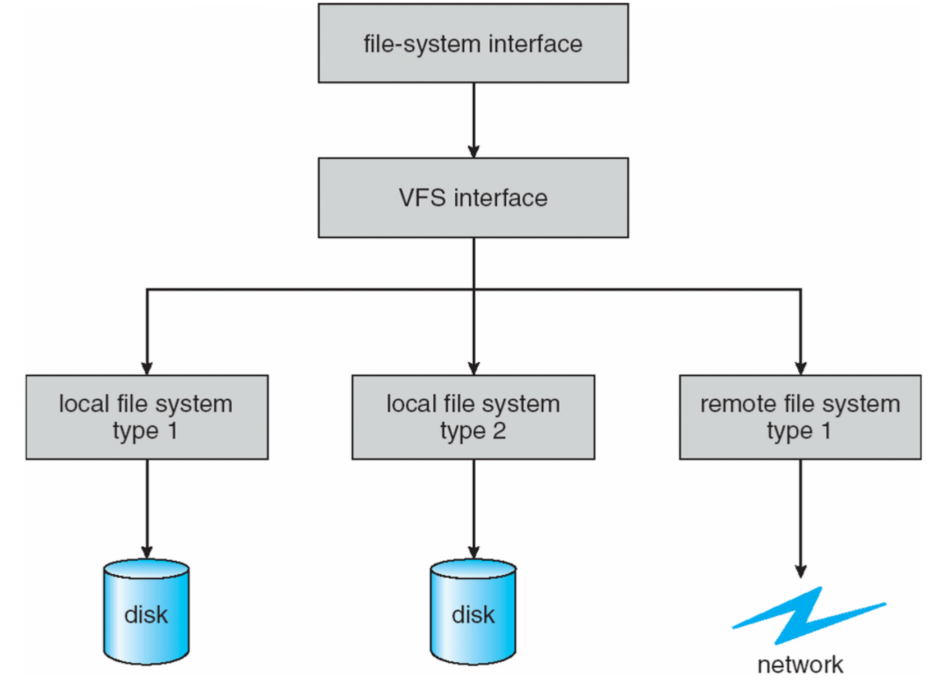
\includegraphics[width=0.33\textwidth]{VirtualFileSystem}\end{figure}

\paragraph{Files --- implementation}
\begin{items}
  \item \textbf{meta data} must be tracked: \\*
    $ - $ which logical block belongs to which file? \\*
    $ - $ block order? \\*
    $ - $ which blocks are free for next allocation?
  \item \textbf{block identification}: blocks on disk must be identified by FS (given logical region of file) \\*
    $ \to $ meta data needed in \emph{file allocation table}, \emph{directory} and \emph{inode}
  \item \textbf{block management}: creating/updating files might imply allocating new/modifying old disk blocks
\end{items}

\paragraph{Allocation --- policies}
\begin{items}
  \item \textbf{preallocation}: \\*
    $ - $ \emph{problem}: need to know maximum file size at creation time \\*
    $ - $ often difficult to reliably estimate maximum file size \\*
    $ - $ users tend to overestimate file size to avoid running out of space
  \item \textbf{dynamic allocation}: allocate in pieces as needed
\end{items}

\paragraph{Allocation --- fragment size}
\begin{items}
  \item \textbf{extremes}: \\*
    $ - $ fragment size = length of file \\*
    $ - $ fragment size = smallest disk block size (= sector size)
  \item \textbf{trade-offs}: \\*
    $ - $ \emph{contiguity}: speedup for sequential accesses \\*
    $ - $ \emph{small fragments}: larger tables needed to manage free storage and file access \\*
    $ - $ \emph{large fragments}: improve data transfer \\*
    $ - $ \emph{fixed-size fragments}: simplifies space reallocation \\*
    $ - $ \emph{variable-size fragments}: minimizes internal fragmentation, can lead to external fragmentation
\end{items}

\paragraph{Allocation --- file space}
\begin{items}
  \item \textbf{contiguous}
  \item \textbf{chained}
  \item \textbf{indexed}: \\*
    $ - $ fixed block fragments \\*
    $ - $ variable block fragments
\end{items}
\begin{figure}[H]\centering\label{AllocationOverview}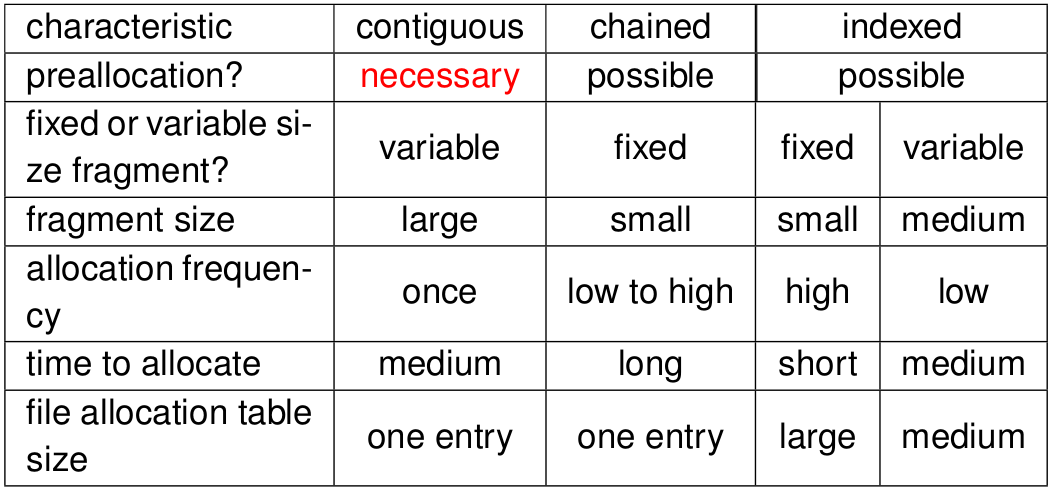
\includegraphics[width=0.33\textwidth]{AllocationOverview}\end{figure}

\paragraph{Allocation --- contiguous}
\begin{items}
  \item \textbf{principle}: array of $ n $ contiguous logical blocks reserved per file (to be created)
  \item \textbf{periodic compaction}: overcome external fragmentation
\end{items}
\begin{figure}[H]\centering\label{AllocationContiguous}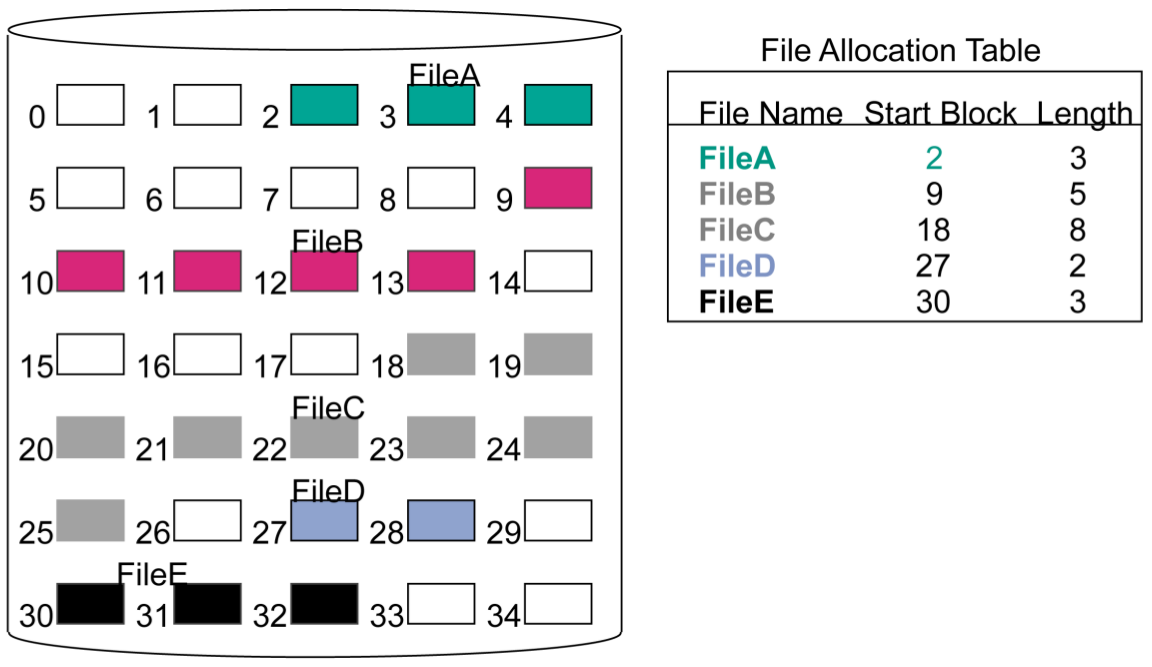
\includegraphics[width=0.33\textwidth]{AllocationContiguous}\end{figure}

\paragraph{Allocation --- chained}
\begin{items}
  \item \textbf{principle}: linked list of logical blocks per file \\*
    $ - $ FAT or directory contains address of first file block \\*
    $ \to $ \emph{no external fragmentation}: any free block can be added to chain
\end{items}
\begin{figure}[H]\centering\label{AllocationChained}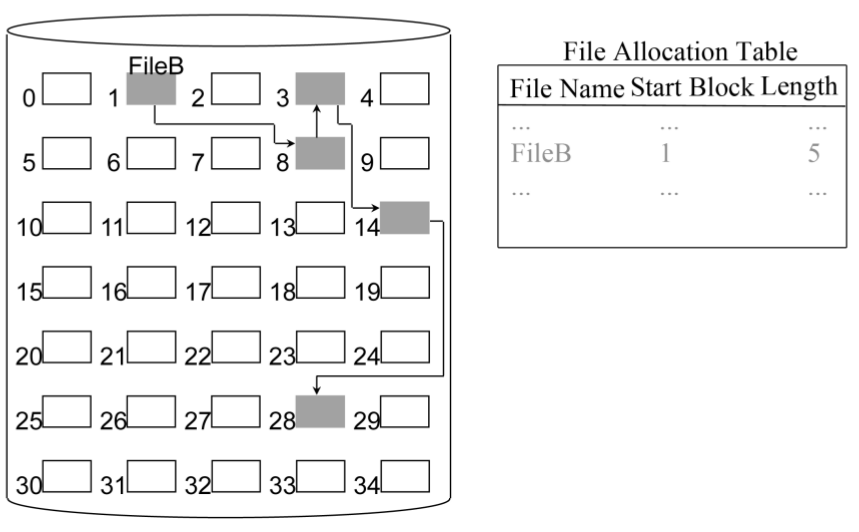
\includegraphics[width=0.33\textwidth]{AllocationChained}\end{figure}

\paragraph{Allocation --- indexed}
\begin{items}
  \item \textbf{principle}: FAT contains one-level index table per file \\*
    $ - $ \emph{generalization}: $ n $-level index table \\*
    $ - $ index has one entry for allocated file block \\*
    $ - $ FAT contains block number for index
\end{items}
\begin{figure}[H]\centering\label{AllocationIndexed}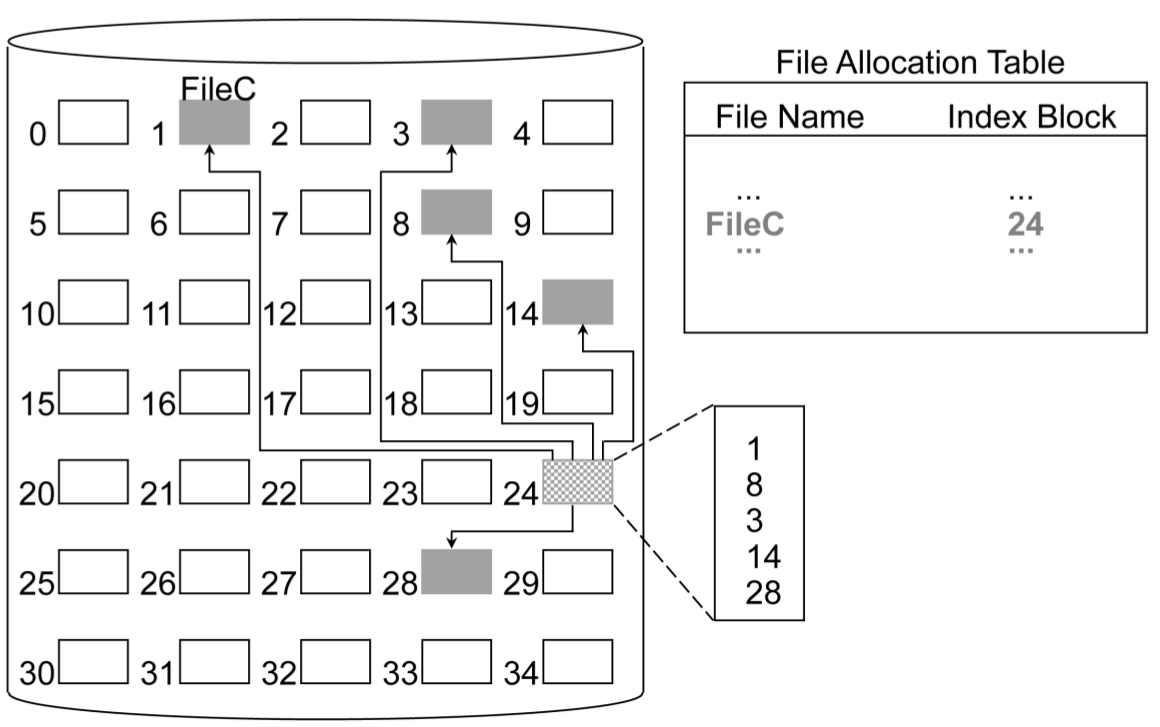
\includegraphics[width=0.33\textwidth]{AllocationIndexed}\end{figure}

\paragraph{Directories --- implementation}
\begin{items}
  \item \textbf{simple directory} (MS-DOS): \\*
    $ - $ fixed-size entries \\*
    $ - $ disk addresses + attributes in directory entry
  \item \textbf{i-node reference directory} (UNIX): \\*
    $ - $ entry refers to i-node containing attributes
\end{items}

\paragraph{Disk Blocks --- buffering}
\begin{items}
  \item \textbf{buffering}: disk blocks buffered in main memory
  \item \textbf{access}: buffer access done via hash table \\*
    $ - $ blocks with same hash value are chained together
  \item \textbf{replacement}: LRU
  \item \textbf{management}: free buffer is managed via doubly-linked list
\end{items}

\paragraph{File Systems --- journaling}
\begin{items}
  \item \textbf{principle}: record each update to file system as \emph{transaction} \\*
    $ - $ written to log
  \item \textbf{committed} transaction = written to log \\*
    $ \to $ \emph{problem}: file system may not yet be updated
  \item \textbf{writing} transactions from log to FS is asynchronous
  \item \textbf{modifying} FS $ \to $ transaction removed from log
  \item \textbf{crash} of file system $ \to $ remaining transactions in log must still be performed
\end{items}

\paragraph{File Systems --- log-structured}
\begin{items}
  \item \textbf{principle}: use disk as circular buffer \\*
    $ - $ write all updated (including i-nodes, meta data and data) to end of log
  \item \textbf{buffering}: all writes initially buffered in memory
  \item \textbf{writing}: periodically write within 1 segment (1 MB)
  \item \textbf{opening}: locate i-node, find blocks
  \item \textbf{clearing}: clear all data from other end, no longer used
\end{items}

  % \section{I/O Systems}

\paragraph{Device Management --- objectives}
\begin{itemize}
  \item \textbf{abstraction} from details of physical devices
  \item \textbf{uniform naming} that does not depend on hardware details
  \item \textbf{serialization} of I/O operations by concurrent applications
  \item \textbf{protection} of standard-devices against unauthorized accesses
  \item \textbf{buffering} if data from/to device cannot be stored in final destination
  \item \textbf{error handling} of sporadic device errors
  \item \textbf{virtualizing} physical devices via memory + time multiplexing
\end{itemize}

\paragraph{Device Management --- techniques}
\begin{itemize}
  \item \textbf{programmed I/O}: \\*
    $ - $ thread is busy-waiting for I/O operation to complete $ \to $ CPU cannot be used elsewhere \\*
    $ - $ kernel is \emph{polling} state of I/O device (command-ready, busy, error)
  \item \textbf{interrupt-driven I/O}: \\*
    $ - $ I/O command is issued \\*
    $ - $ processor continues executing instructions \\*
    $ - $ I/O device sends interrupt when command is done
  \begin{figure}[h]\centering\label{InterruptIO}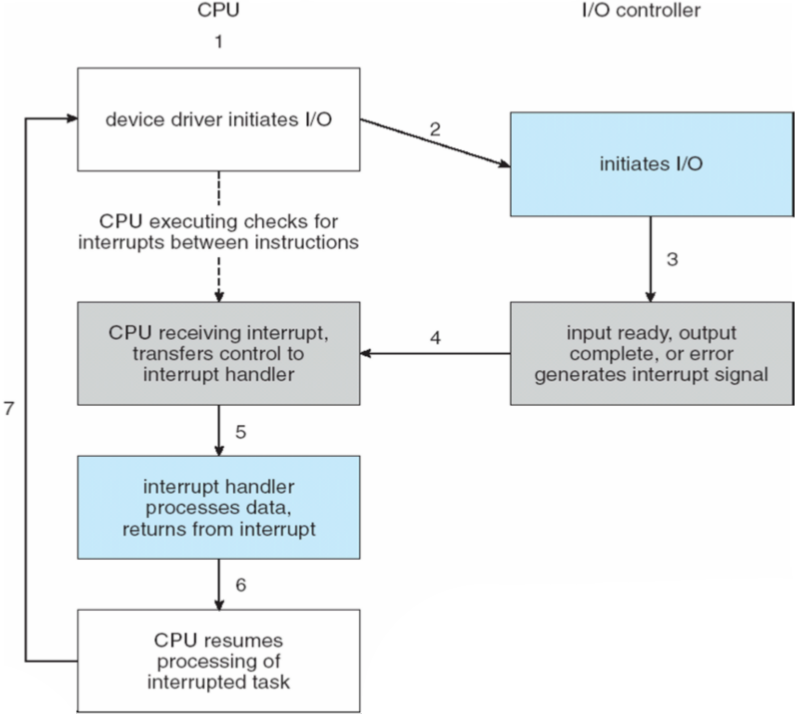
\includegraphics[width=0.33\textwidth]{InterruptIO}\end{figure}
  \item \textbf{direct memory access} (DMA): \\*
    $ - $ DMA module controls exchange of data between main memory and I/O device \\*
    $ - $ processor interrupted after entire block has been transferred \\*
    $ \to $ bypasses CPU to transfer data directly between I/O device and memory
  \begin{figure}[h]\centering\label{DMA}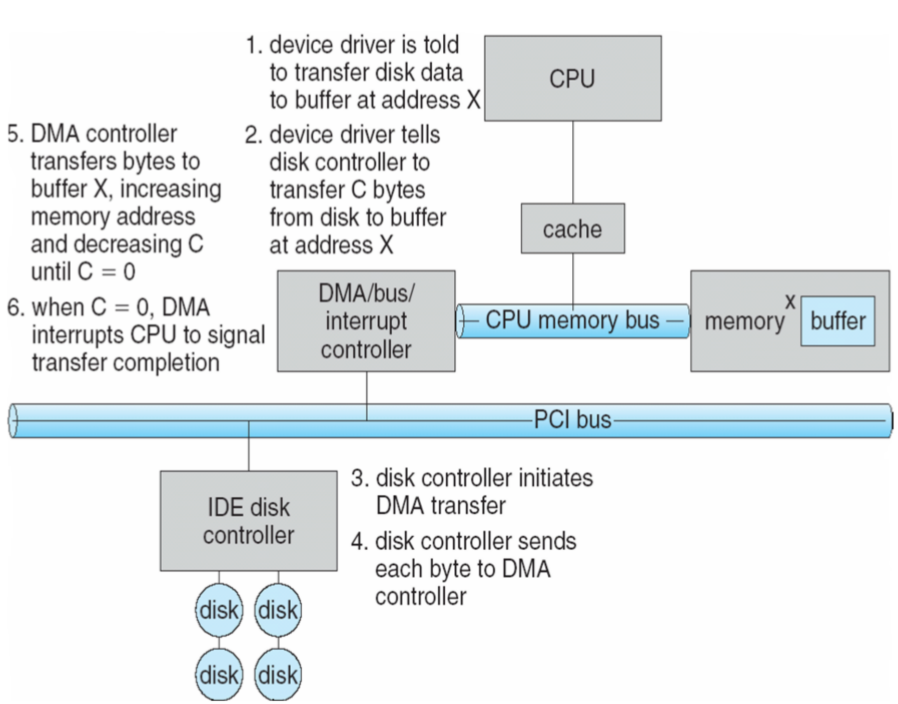
\includegraphics[width=0.33\textwidth]{DMA}\end{figure}
\end{itemize}

\paragraph{Kernel I/O Subsystem}
\begin{itemize}
  \item \textbf{scheduling}: order I/O requests in per-device queues
  \item \textbf{buffering}: store data in memory while transferring between devices
  \item \textbf{error handling}: recover from read/availability/write errors
  \item \textbf{protection}: protect from accidental/purposeful disruptions
  \item \textbf{spooling}: hold output to device if device is slow (e.g., printer)
  \item \textbf{reservation}: provide exclusive access for process
\end{itemize}

\paragraph{Device Drivers}
\begin{itemize}
  \item \textbf{jobs}: \\*
    $ - $ \emph{translate} user request through device-independent standard interface \\*
    $ - $ \emph{initialize} hardware at boot time \\*
    $ - $ \emph{shut down} hardware
\end{itemize}

\paragraph{Device Buffering}
\begin{itemize}
  \item \textbf{reasons}: \\*
    $ - $ without buffering threads must wait for I/O to complete before proceeding \\*
    $ - $ pages must remain in main memory during physical I/O
  \item \textbf{version 1 --- block-oriented}: \\*
    $ - $ information is stored in fixed-size blocks \\*
    $ - $ transfers are made a block at a time \\*
    $ - $ used for disks/tapes
  \item \textbf{version 2 --- stream-oriented}: \\*
    $ - $ transfer information as byte stream \\*
    $ - $ used for keyboard, terminals, \dots (most things that is not secondary storage)
\end{itemize}

\paragraph{Buffering --- user level}
\begin{itemize}
  \item \textbf{principle}: task specifies memory buffer where incoming data is placed
  \item \textbf{issues}: \\*
    $ - $ what happens if buffer is currently paged out to disk? $ \to $ data loss \\*
    $ - $ additional problems with writing? $ \to $ when is buffer available for re-use?
\end{itemize}

\paragraph{Buffering --- single}
\begin{itemize}
  \item \textbf{principle}: user process can process one data block while next block is read in
  \item \textbf{swapping}: can occur since input is taking place in system memory, not user memory
  \item \textbf{stream-oriented}: buffer = input line, carriage return signals end of line
  \item \textbf{block-oriented}: \\*
    $ - $ input transfers made to \emph{system buffer} \\*
    $ - $ buffer moved to \emph{user space} when needed \\*
    $ - $ another block read into system buffer
\end{itemize}

\paragraph{Buffering --- double}
\begin{itemize}
  \item \textbf{principle}: use 2 system buffers instead of 1 (per user process)
  \item user process can write/read from one buffer while OS empties/fills other buffer
\end{itemize}

\paragraph{Buffering --- circular}
\begin{itemize}
  \item \textbf{problem}: double buffer insufficient for high-burst traffic situations: \\*
    $ - $ many writes between long periods of computations \\*
    $ - $ long computation periods while receiving data \\*
    $ - $ might want to read ahead more than just single block from disk
\end{itemize}

  % \section{OS Structures}

\paragraph{Monolithic Systems}
\begin{items}
  \item \textbf{advantages}: \\*
    $ - $ well understood \\*
    $ - $ easy access to all system data (all shared) \\*
    $ - $ low module interaction cost (procedure call) \\*
    $ - $ extensible via interface definitions
  \item \textbf{disadvantages}: \\*
    $ - $ no protection between system and application \\*
    $ - $ not stable/robust
\end{items}

\paragraph{Layered Systems}
\begin{items}
  \item \textbf{principle}: system is divided into many \emph{layers}: \\*
    $ - $ \emph{each layer} uses functions and services of lower levels \\*
    $ - $ \emph{bottom layer} = hardware \\*
    $ - $ \emph{top layer} = user interface \\*
    $ - $ \emph{lower layers}: implement mechanisms \\*
    $ - $ \emph{higher layers}: implement policies (mostly)
  \item \textbf{advantages}: \\*
    $ - $ \emph{modular}: each layer can be tested/verifies independently \\*
    $ - $ \emph{correctness} of layer $ n $ only depends on layer $ n-1 $ $ \to $ simple debugging/maintenance
  \item \textbf{disadvantages}: \\*
    $ - $ just unidirectional protection \\*
    $ - $ mutual dependencies prevent strict layering
\end{items}

\paragraph{Monolithic Kernels}
\begin{items}
  \item \textbf{advantages}: \\*
    $ - $ well understood \\*
    $ - $ performance OK \\*
    $ - $ sufficient protection between applications \\*
    $ - $ extensible via definitions + static/loadable modules
  \item \textbf{disadvantages}: \\*
    $ - $ no protection between kernel components \\*
    $ - $ side-effects by undocumented interfaces \\*
    $ - $ complexity due to high degree of interdependency
\end{items}

\paragraph{Micro-Kernels}
\begin{items}
  \item \textbf{advantages}: \\*
    $ - $ easier to test/prove/modify \\*
    $ - $ improved robustness/security \\*
    $ - $ improved maintainability \\*
    $ - $ coexistence of several APIs \\*
    $ - $ natural extensibility
  \item \textbf{disadvantages}: \\*
    $ - $ additional decomposing \\*
    $ - $ low performance due to communication overhead
\end{items}

\paragraph{Virtual Machines}
\begin{items}
  \item \textbf{principle}: takes layered approach to logical conclusion --- treats hardware + OS kernel as like they were hardware
  \item VM provides \emph{identical} interface to underlying bare hardware
  \item OS host creates illusion that process has own processor, memory,\dots
  \item each guest gets (virtual) copy of underlying computer
  \item \textbf{benefits}: \\*
    $ - $ multiple execution environments can share same hardware \\*
    $ - $ protection \\*
    $ - $ controllable file sharing \\*
    $ - $ use networking to communicate with each other \\*
    $ - $ useful for development/testing
\end{items}

\end{document}